% chapter3 模型

\chapter{基于特征融合和注意力机制的运动想象脑电图分类网络构建}

论文前两个章节主要对运动想象脑电图(Motor Imagery Electroencephalography,MI-EEG)分类领域的基础知识以及相关研究做了一定的介绍,并且对该领域仍然存在的问题进行了分析。本章对这些问题进行进一步的探讨,针对这些问题提出了一种端到端的新模型HA-FuseNet:首先,在Inception模型的基础上引入密集连接,在进行多尺度特征提取的同时,对EEG信号的浅层特征和高级语义信息加以利用,以更完整地获取EEG信号的特征;其次,在以上结构的基础上,针对EEG信号的特性构建了svSE混合注意力模块,将方差信息和时空轴向分离引入注意力机制中,提高模型对EEG信号中的重要特征的关注度;随后,针对EEG信号的时序特性,使用LSTM获取长短期时序依赖,同时,构建了全局自注意力模块SCoT以更好地利用EEG信号的全局时空信息;最后,为了取得更好的实时性能,对模型进行了轻量化设计。经过以上构建,HA-FuseNet能够同时利用EEG信号的局部特征细节和全局依赖信息,实现更为丰富的特征融合效果,获得更好的MI-EEG分类效果。

\section{基于特征融合和注意力机制的端到端MI-EEG分类网络HA-FuseNet}

原始的EEG信号通常为二维数据,包括通道(电极)和时间两个维度,具体而言,在EEG信号矩阵中,行代表分布在头皮不同位置的采样通道,列为时间序列数据,每个采样点对应一个时间戳下的生物电信号(通常为电压值),因此,一列数据就是一个特定时间点下所有通道同步采集到的电压读数。原始的EEG信号经过预处理之后,可以转换为时频图、头皮点位拓扑图等输入模式,尽管经过转换的输入相较于原始输入能够更全面地体现EEG信号的时频空信息,但这一过程往往需要具有神经科学背景的人工参与,在增加了人工成本同时,限制了模型自适应学习EEG信号中蕴含的复杂时空特征的能力,此外,复杂的预处理环节也增加了计算开销和应用成本,难以满足BCI系统即时响应的需求。因此,端到端网络在MI-EEG分类领域受到越来越多的重视,这类网络不经过或者仅仅经过很少的预处理步骤,而由深度学习算法自适应地提取关键特征并作出预测。

为此,论文构建了基于特征融合和注意力机制的端到端MI-EEG分类网络HA-FuseNet,其结构如图所示。HA-FuseNet有两条并行分支,分别是基于卷积神经网络搭建的分支与基于长短期记忆网络的分支。卷积神经网络分支基于Inception结构搭建,通过在Inception分支引入密集连接结构,进行多尺度特征提取,同时利用高级语义信息与浅层特征;通过引入反转瓶颈层,在深度维度上促进时空特征的融合;通过引入svSE混合注意力模块促进网络对重要特征的关注度,svSE模块采取时空特征分离的策略,同时利用了EEG信号的方差信息,以获得针对性的结果。长短期记忆网络分支用以获取时间域的长期依赖信息,并且加入了SCoT全局注意力模块获取时空域的全局上下文信息。双分支的特征通过C2R模块和R2C模块进行交互,并随后在深度维度进行融合,以在利用卷积神经网络提取到的局部信息的同时有效地建立全局依赖关系,从而获取更为精准的分类效果。

通过HA-FuseNet,可以更完整地获取MI-EEG信号的有效特征,提升分类效果。在下文中,将依次阐述论文的改进思路与构建方法。

\section{基于多尺度密集连接和混合注意力的分类网络DIS-Net}

卷积神经网络具有强大的特征提取能力,在计算机视觉等领域应用广泛。EEG信号在时空域上具有局部相关性,即相邻的电极点和相近的时间窗内的信号往往携带相似的信息(但数据中相邻的行未必在空间域中相邻),因此,可以将EEG信号视为二维图像,使用卷积神经网络提取其局部特征。

\subsection{基于Inception的基础网络}

ShallowConvNet\cite{schirrmeister2017deep}是一个专为端到端解码脑电图(EEG)信号而设计的深度学习架构,其构思源自EEG信号解码研究领域中广泛使用的经典特征提取方法——滤波器组共空间模式(Filter Bank Common Spatial Pattern, FBCSP)\cite{ang2008filter}。ShallowConvNet具有FBCSP算法对频带功率特征高效提取的特性,在实验中证明了能够学习频带功率变化的时间结构特性\cite{schirrmeister2017deep},研究发现,该特性有助于提高分类性能\cite{sakhavi2015parallel}。实验证明,ShallowConvNet在MI-EEG分类领域具有优良的性能\cite{lawhern2018eegnet},其采用四步流程对原始二维输入数据进行处理。具体而言,ShallowConvNet首先通过时间卷积层捕获信号的时间域特征,再通过空间卷积层捕获这些时间特征在不同通道间的空间关联性,随后通过平均池化层进行下采样,最后通过全连接层将多维特征映射至分类输出空间。ShallowConvNet提出的时间卷积与空间卷积相分离的策略是由于EEG原始输入的时域与空域之间的相关性较低,后续的研究大多沿袭了这种方法,论文同样遵循这一思路对EEG信号进行处理。

将EEG原始输入视为具有空间信息的图像数据,论文参考以下几种计算机视觉领域的经典模型,用于网络的特征提取基础结构:

(1) Inception网络

Inception模块起源于经典的GoogLeNet模型\cite{szegedy2015going},并在计算机视觉图像分类任务中取得了优异的效果。传统卷积神经网络倾向于通过加深和拓宽网络结构以增进性能,然而这种做法伴随着参数数量的激增,不仅加大了计算负担,还可能导致过拟合问题。在这种背景下,Inception模块提出了多尺度特征并行抽取的策略,旨在保持网络稀疏性的同时,充分利用密集矩阵运算的高性能。典型的Inception-V1模块的结构如图~\ref{fig:Inception}~所示,其将不同大小的卷积层和最大池化层并行排列,并行地对输入数据执行多种卷积和池化运算,继而将提取到的不同尺度特征在深度维度上进行拼接。这种设计能够在单层网络内并行地提取输入数据在不同层次和粒度的特征信息,从而在高效扩展网络的深度和宽度的同时,有效削减参数规模,提升计算速度。此外,Inception模块中引入了\(1\times1\)卷积核,用以实现深度上的特征转化和降维,这种方式能够让模型学习到更为丰富的特征,同时降低计算成本。后续的论文中,Inception模块不断迭代优化,陆续引入了批归一化、深度可分离卷积、矩阵因子分解等技术,进一步提升了模型的性能\cite{szegedy2016rethinking}\cite{szegedy2017inception}。
\begin{figure}
  \centering
  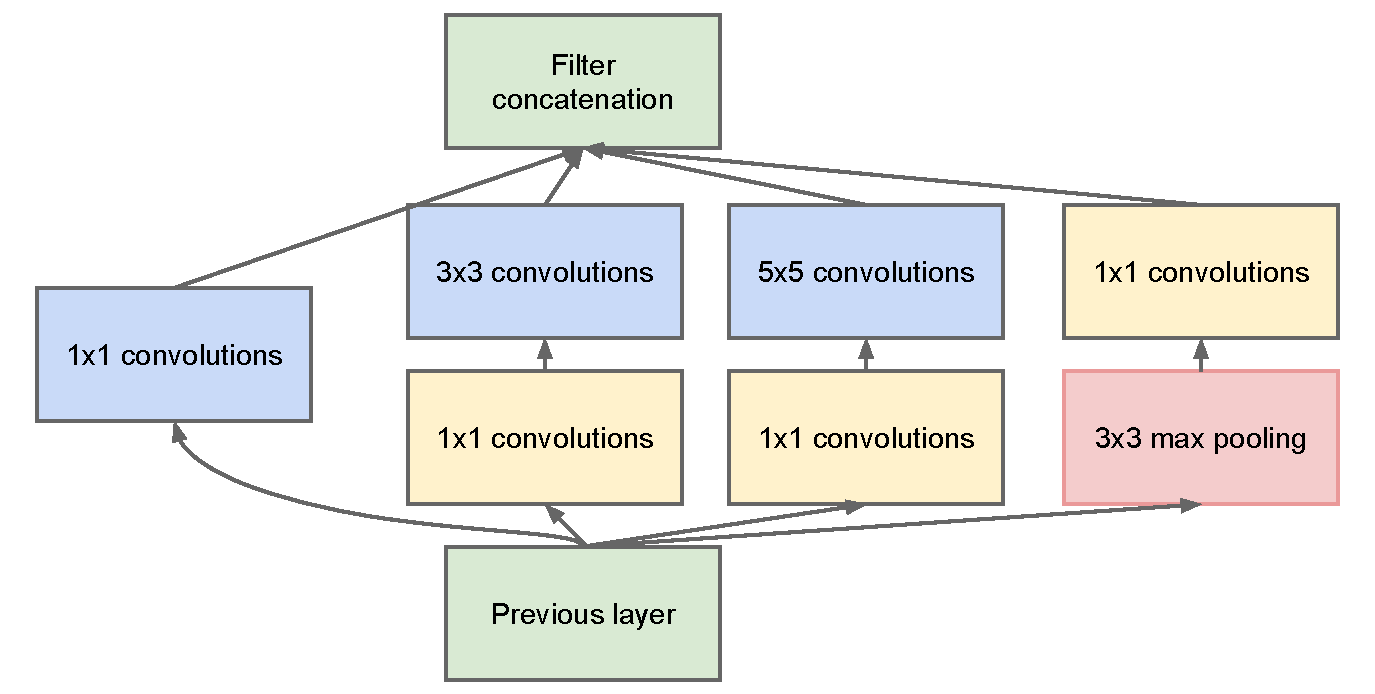
\includegraphics[width=0.6\textwidth]{Inception.pdf}
  \caption{Inception结构\cite{szegedy2015going}}
  \label{fig:Inception}
\end{figure}

(2) 残差神经网络

残差神经网络(Residual Network,ResNet)\cite{he2016deep}是计算机视觉图像识别领域的一个经典模型。ResNet研究发现了深度神经网络的退化现象(Degradation),即随着网络深度不断增加,模型准确率起初随深度上升,却在达到峰值后急剧下滑。针对这种现象,ResNet提出了残差学习框架,其核心思想是引入残差块(Residual Block),每个残差块通过快捷连接(Shortcut Connection)将输入信息直接输送至输出层,使得网络只需要专注学习输入与输出之间的残差信息,而非完整的映射关系。基础的ResNet由一系列残差块堆叠而成,残差块的结构如图~\ref{fig:ResNet}~所示。通过快捷连接,ResNet在训练过程中,梯度能够从深层网络直接回传至浅层,避免网络深度增加带来的训练困难和性能下降问题,从而提升深度神经网络的性能表现和训练效率。
\begin{figure}
  \centering
  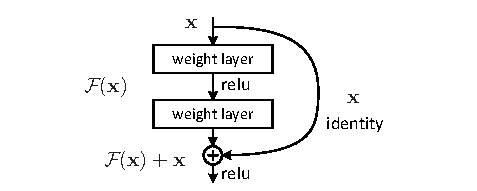
\includegraphics[width=0.6\textwidth]{ResNet.pdf}
  \caption{残差块结构\cite{he2016deep}}
  \label{fig:ResNet}
\end{figure}

(3) U-Net

U-Net模型\cite{ronneberger2015u}最初是为生物医学图像分割任务而设计,其具有优秀的性能,尤其在细胞、器官和病变区域的精确标注上表现出色,是医学图像分割领域的主流模型之一。U-Net的独特之处在于其采用了对称的编码-解码结构(Encoder-Decoder)和跳跃连接(skip connection),其结构如图~\ref{fig:UNet}~所示。编码器通过连续的卷积和下采样层对输入图像进行深度特征提取和空间压缩,提炼出高级抽象特征;解码器部分则通过上采样和卷积恢复到与输入图像相同的空间分辨率,同时保留详细的定位信息。跳跃连接将编码器各阶段的特征图直接传递给相应的解码器阶段,有效地结合了包含更多细节信息的浅层特征和包含更多高级语义信息的深层特征,从而在图像分割任务中能够取得更为精细的分割效果。同时,U-Net模型结构简单,易于训练,能够缓解小样本数据集上的过拟合问题。
\begin{figure}
  \centering
  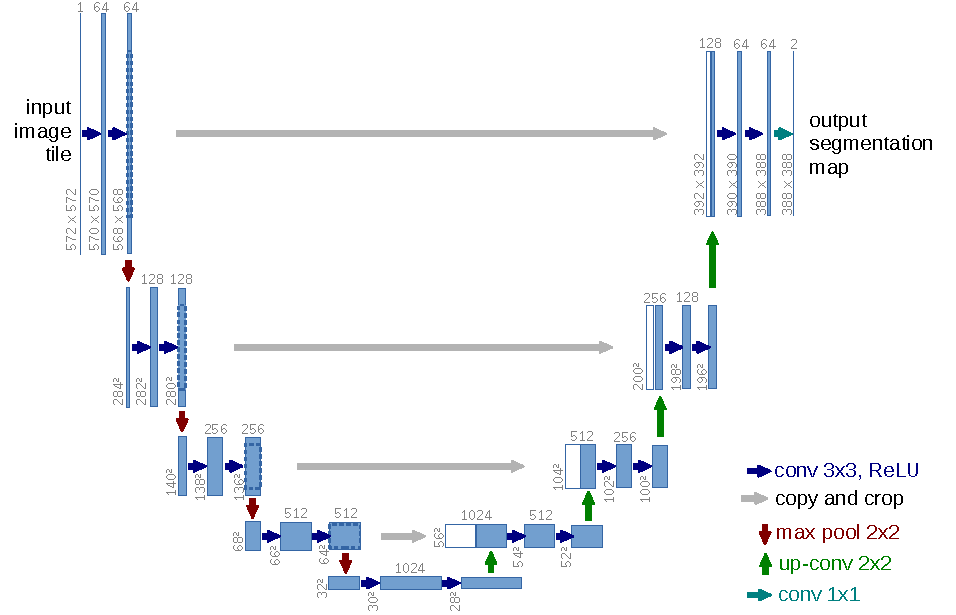
\includegraphics[width=0.6\textwidth]{UNet.pdf}
  \caption{U-Net结构\cite{ronneberger2015u}}
  \label{fig:UNet}
\end{figure}

在这三种模型中,Inception和ResNet均在图像分类任务中展现出了优秀的性能。Inception通过同一层网络内的多尺度特征并行抽取,在不显著增加网络深度的前提下,实现了特征提取的广度与效率的提升。ResNet通过引入快捷连接,解决了深度神经网络训练过程中的梯度消失和退化问题,增强了深层次网络的训练效率和性能表现。U-Net则在生物医学图像分割领域取得了优秀的表现,医学图像的语义信息较为简单,且结构较为固定,因此高级语义信息和低级特征都相对重要,U-Net通过跳跃连接保留并融合了这两类信息,同时,U-Net参数量较小,不容易在小样本数据集上发生过拟合现象。论文选择将U-Net迁移至MI-EEG分类任务中,是因为EEG信号具有与生物医学图像类似的生理特性,如特征相对简单、数据集规模偏小等。

为了验证Inception、ResNet与U-Net在EEG信号分类任务中的性能,论文在BCI Competition IV Dataset 2A数据集上进行实验对比。在实验设置中,统一将三种模型的网络深度调整为三层,并对其他关键参数如卷积核大小、学习率等进行了固定,此外,对这三种模型的原始代码进行了调整,使得其适应MI-EEG分类任务。实验结果如表~\ref{tab:Incep-Res-U}~所示,主要展示准确率(Accuracy,ACC)和Kappa一致性系数(Kappa)指标,这两项指标是数据集中九位被试的平均表现。
\begin{table}[ht]
  \centering
  \caption{Inception、ResNet、U-Net实验结果对比}
  \label{tab:Incep-Res-U}
  \begin{tabularx}{\textwidth}{CCC}
    \toprule
    Models & ACC(\%) & Kappa \\
    \midrule
    Inception & \textbf{67.40} & \textbf{0.56} \\
    ResNet & 56.94 & 0.43 \\
    U-Net & 62.27 & 0.50 \\
    \bottomrule
  \end{tabularx}
\end{table}

实验数据显示,Inception模型在这三种模型中具有最优的性能表现,U-Net次之,ResNet的表现则相对较差。这可能是因为同样的网络深度下,Inception模型得益于多尺度并行特征提取机制,能更全面地捕获EEG信号的多种特征。相比之下,U-Net虽然通过跳跃连接有效地结合了EEG信号的低层特征和高层语义信息,但在解码器阶段,U-Net将特征图重建至原始空间尺寸的过程可能为分类任务引入了不必要的复杂性。ResNet的快捷连接在较浅层网络结构中可能未能完全发挥其优势,更适用于深层次网络。实验结果与过往研究中关于浅层网络更适合MI-EEG分类任务的研究结论相互印证。综上所述,论文选用Inception模块作为MI-EEG信号特征提取的基础结构,旨在保持模型简洁高效的同时,在MI-EEG分类任务中取得更好的性能。

EEG信号的空间分辨率较为不稳定,例如,在BCI Competition IV Dataset 2B\cite{tangermann2012review}数据集中,仅仅使用了三个电极采集MI-EEG信号,使得空间信息相对时间信息更为稀疏。为了减少对高空间分辨率的依赖,论文采取更关注时间特征的策略,即将Inception模块应用于时间卷积层中,使得时间卷积层的复杂度高于空间卷积层的复杂度,从而保持相对均衡的特征提取。

文献\cite{schirrmeister2017deep,lawhern2018eegnet}指出,在EEG信号解码任务中,增加神经网络的深度有利于提升解码精度。瓶颈层(Bottleneck Layer)是深度神经网络中的常见结构\cite{he2016deep,huang2017densely},通常用于对数据的降维和升维,由于采用了\(1\times1\)卷积进行操作,瓶颈层能够有效地减少神经网络的参数。不同于原始Inception模块中通过瓶颈层进行数据降维的操作,论文使用瓶颈层对数据进行升维操作,并将瓶颈层提取至卷积和池化操作之前,其目标为在深度维度上促进时空信息的融合。此外,论文在模型中引入了批量归一化层和Dropout层,用以加快网络训练速度,并避免小数据集下过早的过拟合。

论文将改进后得到的基础模型称为BaseNet,其结构如图~\ref{fig:BaseNet}~所示。需要注意的是,Inception模块的层次数量和分支数量是影响其性能表现的两项可调的超参数。
\begin{figure}
    \centering
    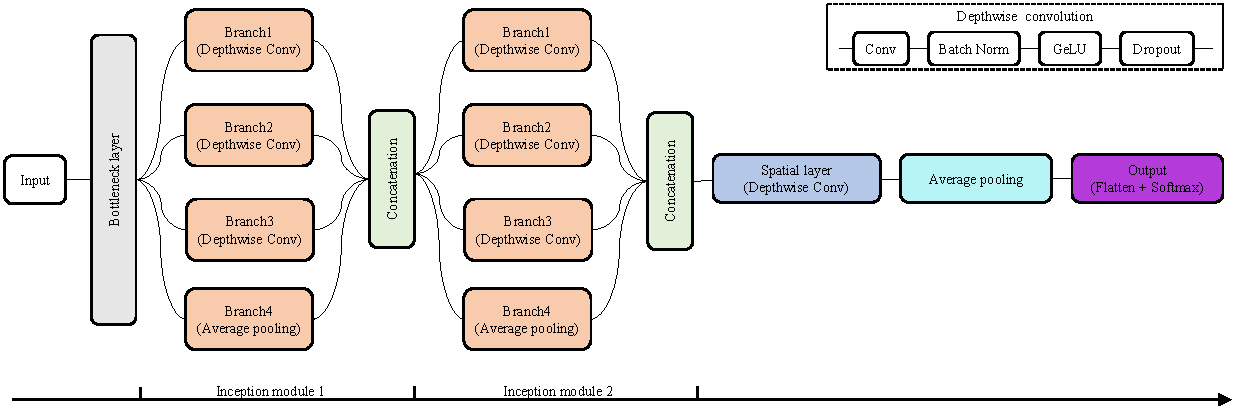
\includegraphics[width=\textwidth]{Base-Net.pdf}
    \caption{BaseNet结构}
    \label{fig:BaseNet}
\end{figure}

\subsection{多尺度密集连接}

在构建BaseNet时,论文发现U-Net在处理MI-EEG分类任务时同样展现了一定的优势。由于EEG信号的特征相对简单,因此低级特征与高级语义信息都相对重要,U-Net因其特殊的跳跃连接结构有效地融合了这两种信息,然而,U-Net中通过解码器阶段将特征图恢复至原始空间尺寸的操作并非必要,因为在分类任务中,这种重建过程可能导致额外的计算负担且对分类性能的提升效果不明显。因此,论文从U-Net兼顾低级特征与高级语义信息的策略中得到启发,同时对不必要的特征图空间尺寸还原过程进行规避,以构建一个既能充分利用EEG信号中各级别特征信息,又具备高效计算能力的改进模型。

Gao Huang等人于2016年提出了密集连接网络\cite{huang2017densely}(Dense Convolutional Network,DenseNet)。在ResNet的基础上,DenseNet提出了一种更为激进的连接模式:引入从任意层到后续层的直接连接,即密集连接(Dense Connection)。DenseNet的第 \(l\) 层接收所有前序特征图为输入,其输出为 \(x_l\):
\begin{equation}
  x_l = H_l([x_0, x_1, ···, x_{l-1}])
  \label{eq:dense-conn}
\end{equation}
其中,\([x_0, x_1, ···, x_{l-1}]\) 代表第 \(0, ···, l-1\) 层的输出特征图,\(H_l(·)\) 代表非线性转换复合函数,可能包括一系列的批量归一化、ReLU、池化及卷积操作。密集连接的结构如图~\ref{fig:denseBlock}~所示。
\begin{figure}
  \centering
  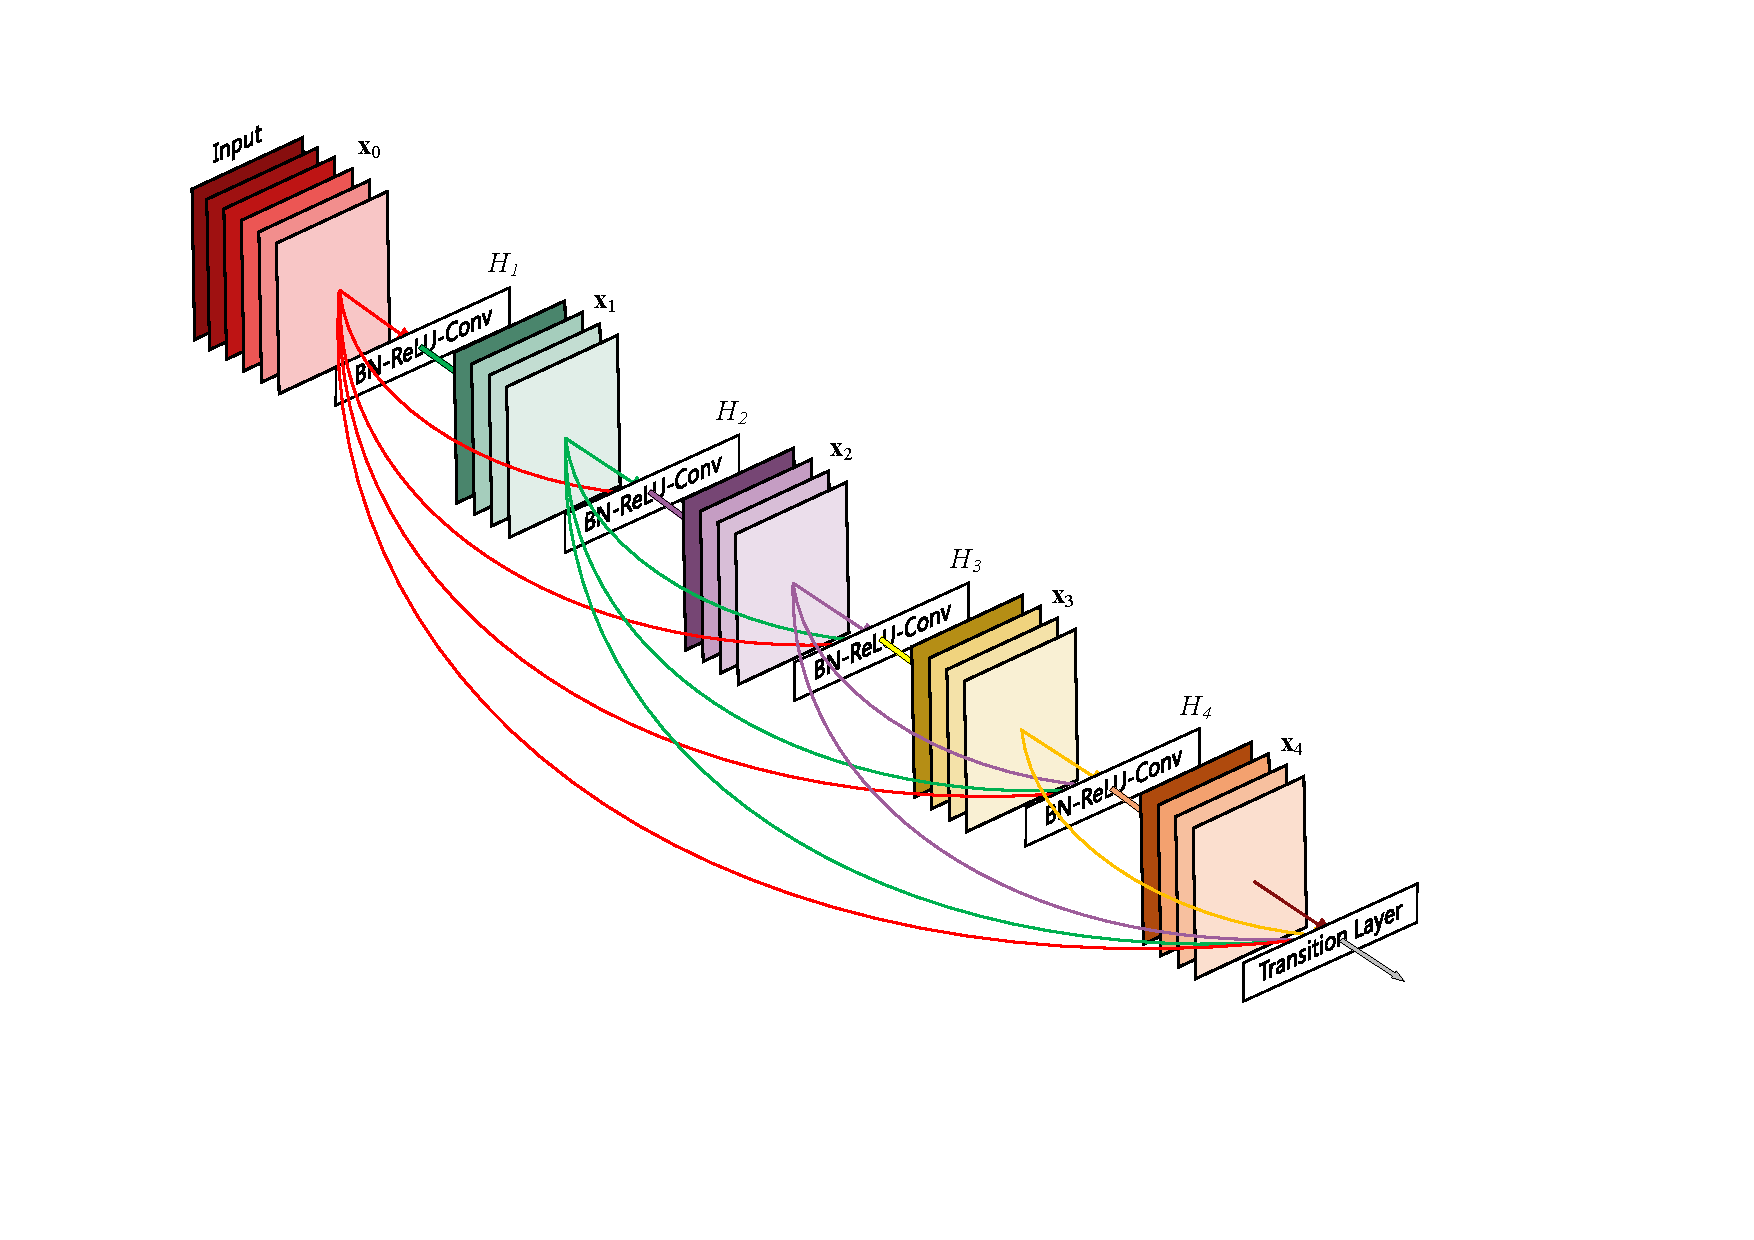
\includegraphics[width=0.5\textwidth]{denseBlock.pdf}
  \caption{密集连接结构\cite{huang2017densely}}
  \label{fig:denseBlock}
\end{figure}

在密集连接模块中,所有的前序特征图通过Concentrate在深度维度上连接在一起,因此,在一个密集连接模块中所有特征图的大小是相同的。DenseNet提出了Transition模块用于连接两个相邻的密集连接模块,并通过池化操作对特征图进行下采样,从而减小特征图的大小。

通过密集连接的方式,网络中的每一层都能够访问并整合所有前序层提取出的特征信息,进而充分利用EEG信号中的低层特征细节和高层语义信息。相较于U-Net中的编码-解码结构,密集连接无需经历数据空间的重建过程,即可实现特征的有效复用。此外,DenseNet中的Transition模块也为实现特征图的下采样提供了思路。

为了同时利用Inception模块多尺度并行特征提取和密集连接兼顾深层与浅层特征的优点,论文选择将DenseNet嵌入Inception模块中,替代原本的时间卷积核。为了简洁起见,下文称之为密集连接模块。

原始的密集连接模块在计算机视觉图像分类任务中都取得了优秀的表现,在设计上,它考虑到了图像数据在空间维度上的局部相关性,然而,EEG信号的时空域局部相关性较低,需要对始密集连接模块的卷积核进行改造。研究指出\cite{lawhern2018eegnet},当设计用于提取EEG特征的卷积核时,将时间卷积核长度设置为EEG信号采样率的一半,可以有效地捕获2Hz及以上频段的信号信息。因此,在处理EEG信号时,时间卷积核的长度应当依据EEG信号的实际采样率来灵活设定,以便提取不同频率成分的信号特征。

将密集连接模块中的卷积核概念转化为针对时间序列的一维卷积(尽管在实现时仍采用二维卷积),为了更好地匹配EEG信号的采样特性及其内在频率成分,依据EEG信号的采样频率 \(sfreq\) 来动态调整位于Inception第 \(i\) 个分支上的密集连接模块的时间卷积核大小 \(kernel_i\),具体公式如下:
\begin{equation}
    kernel_i = \left \lfloor \frac{sfreq}{2 \times i} \right \rfloor , \quad i \le 5
    \label{eq:kernel_cal}
\end{equation}
其中,\(sfreq\) 是EEG信号的采样频率。这样设置卷积核大小是为了更全面地捕捉EEG信号中不同频率成分的特征信息,同时避免因卷积核大小过于接近而导致提取的特征之间重叠度过高。例如,当\(i=1\)时,卷积核大小将是采样率的一半,进而能够有效地捕获到2Hz及更高频段的EEG信号特征。

由此,密集连接模块的非线性转换复合函数 \(H(·)\) 定义如公式~\ref{eq:dense-kernel}所示,
\begin{equation}\label{eq:dense-kernel}
    H(·) = BN + GELU + 1 \times kernel_i\;conv + Dropout 
\end{equation}
经过以上改进,新构建模型的结构如图~\ref{fig:incep-dense}~所示,将其命名为DI-Net。Dense-Inception module构成了时间卷积层,其内部的各个分支均由一系列改进版的Bottleneck Dense Block紧密堆叠而成,形成密集连接结构,用以同时获取浅层和深层的时间特征。每个分支提取的特征图在深度维度上进行聚合,并通过Transition模块进行深度压缩和特征整合,以进一步提升模型的表达能力和计算效率。
\begin{figure}
  \centering
  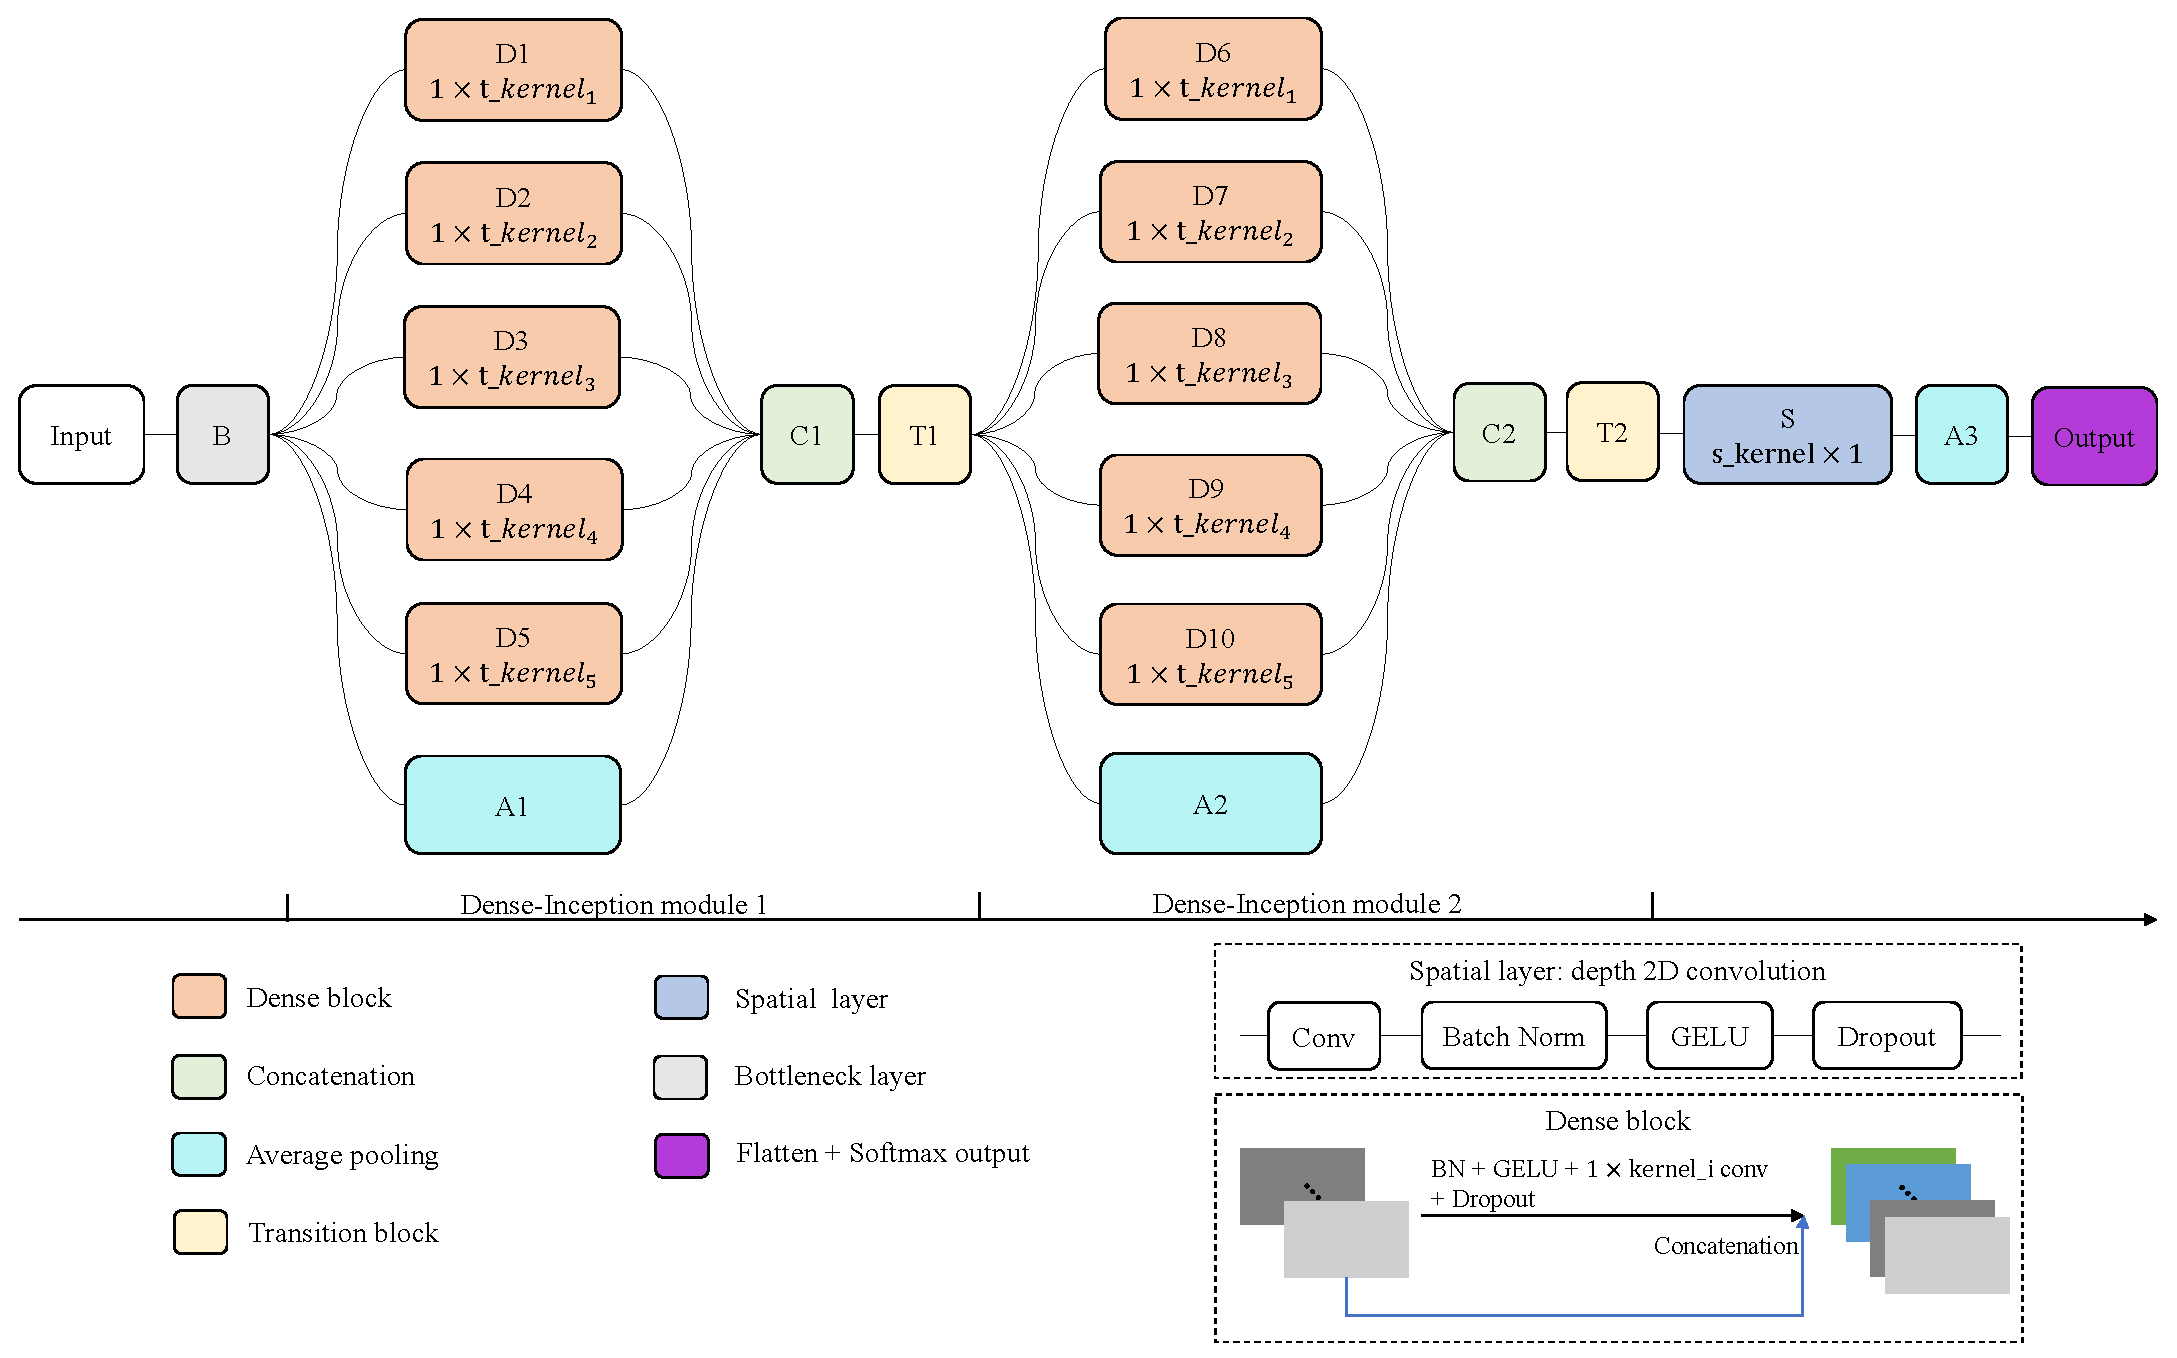
\includegraphics[width=\textwidth]{incep-densev2.pdf}
  \caption{DI-Net结构}
  \label{fig:incep-dense}
\end{figure}

\subsection{混合注意力svSE}

根据神经科学先验知识,EEG信号中不同的通道和采样点具有不同的重要性,这为在MI-EEG分类领域应用注意力机制提供了理论依据,此外,将二维EEG信号视为一种由通道和时间两个维度构成的特殊图像,使得在MI-EEG分类领域能够迁移应用计算机视觉领域中的注意力机制。

计算机视觉领域中经常使用的注意力机制有:

(1) 通道注意力机制
    
不同于EEG信号中代表电极的通道,计算机视觉领域的通道代表图像的不同特征映射。通道注意力机制用于调整不同特征通道的重要性,通常会对每一个特征通道计算一些全局统计量,如均值、方差等,再将这些统计量经过非线性变换层进行编码,最后将编码向量进行转换并用于各个特征通道的加权。通道注意力机制的经典模型是压缩和激励网络(Squeeze-and-Excitation Networks,SENet)\cite{8578843},其主要思想即是压缩(Squeeze)和激励(Excitation),SENet首先通过压缩操作获取全局上下文信息,然后通过激励操作对每个通道独立生成权重系数。具体而言,在压缩操作中,SENet在空间维度执行全局池化操作,将每个通道的特征图汇总成一个标量值;然后,在激励操作中,SENet通过一个全连接网络生成每个通道的权重系数,这些权重系数用于重新加权每个通道的特征图,以增强有用的特征并抑制无用的特征。

在后文中,为避免与计算机视觉领域中的概念相混淆,在MI-EEG分类任务中,用深度来代表EEG信号的不同特征映射,而通道仍然代表电极。

(2) 空间注意力机制
    
在计算机视觉领域中,空间注意力机制用于调整图片、视频等输入数据在空间维度中不同区域的重要性,通常会在深度维度上通过全局池化、卷积、特征融合等操作生成一个与特征图尺寸相同的注意力图,其值反映了空间维度中不同区域的注意力强度,最后,将注意力图进行转换,并用于原始特征图的加权。空间注意力机制的经典模型是空间变换网络(Spatial Transformer Network,STN)\cite{jaderberg2015spatial},其具有对输入数据进行空间变换的能力,能够自动捕获重要区域的特征。

(3) 混合注意力机制
    
混合注意力机制是一种集成多种注意力机制(如空间注意力、通道注意力及自注意力等)的方法,旨在更全面地捕获和整合输入数据在不同维度的有效信息。混合注意力机制通常会使用不同的注意力机制分别计算原始特征图的注意力权重,再将这些注意力权重进行融合,最后将融合后的注意力权重用于原始特征图的加权,或者将不同的注意力权重用于原始特征图加权,再将加权特征图进行融合。混合注意力机制的经典模型有卷积注意力机制模块(Convolutional Block Attention Module,CBAM)\cite{woo2018cbam}、空间与通道压缩与激励模块(Spatial and Channel Squeeze-and-Excitation,scSE)\cite{roy2018concurrent}等。
    
CBAM结合了通道注意力机制与空间注意力机制,其结构如图~\ref{fig:CBAM}~所示,输入特征图首先经过通道注意力模块进行加权,再通过空间注意力模块进行加权,从而得到最终结果。
\begin{figure}
    \centering
    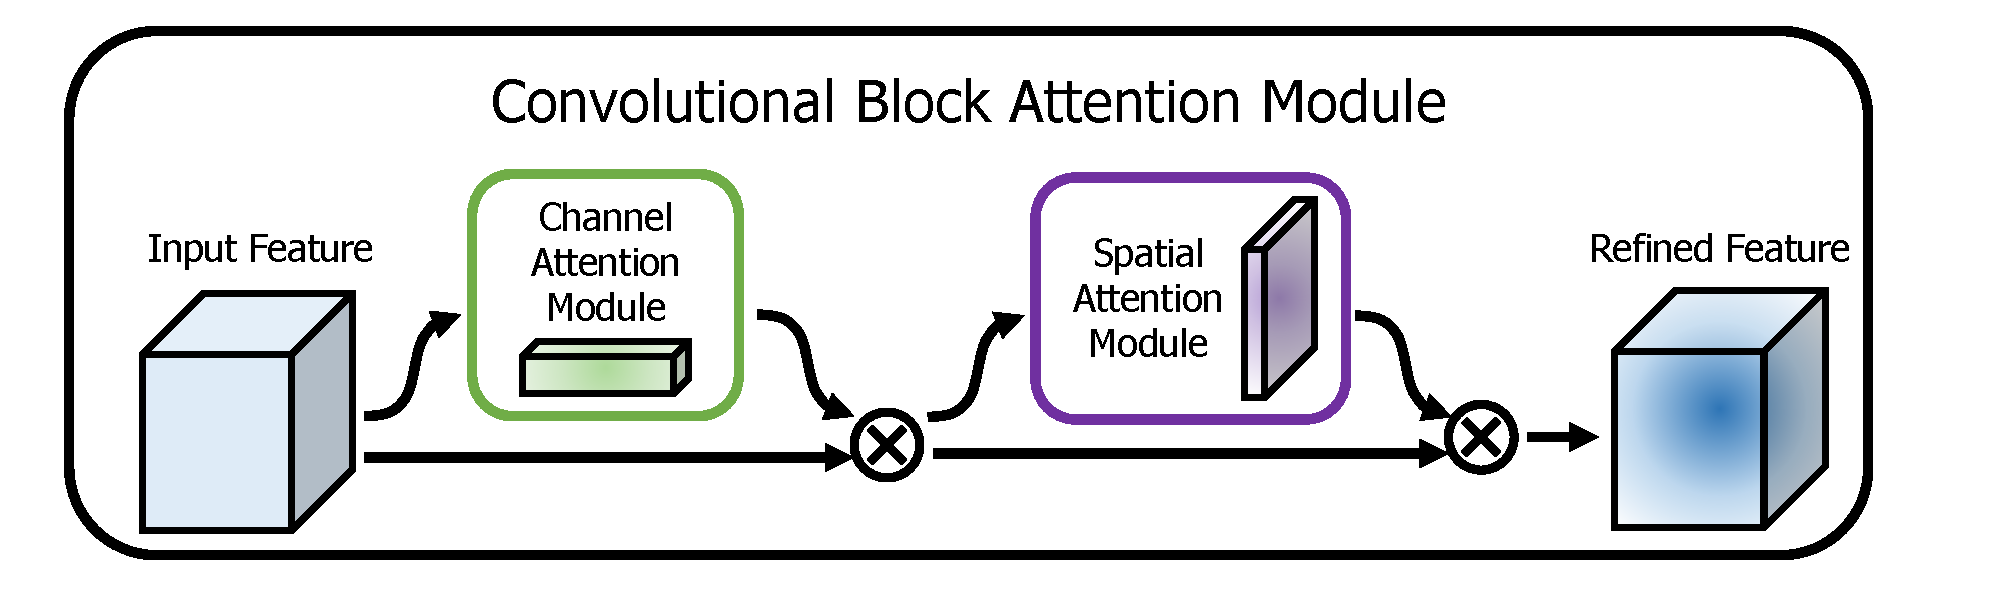
\includegraphics[width=0.6\textwidth]{CBAM.pdf}
    \caption{CBAM结构\cite{woo2018cbam}}
    \label{fig:CBAM}
\end{figure}
\begin{figure}
    \centering
    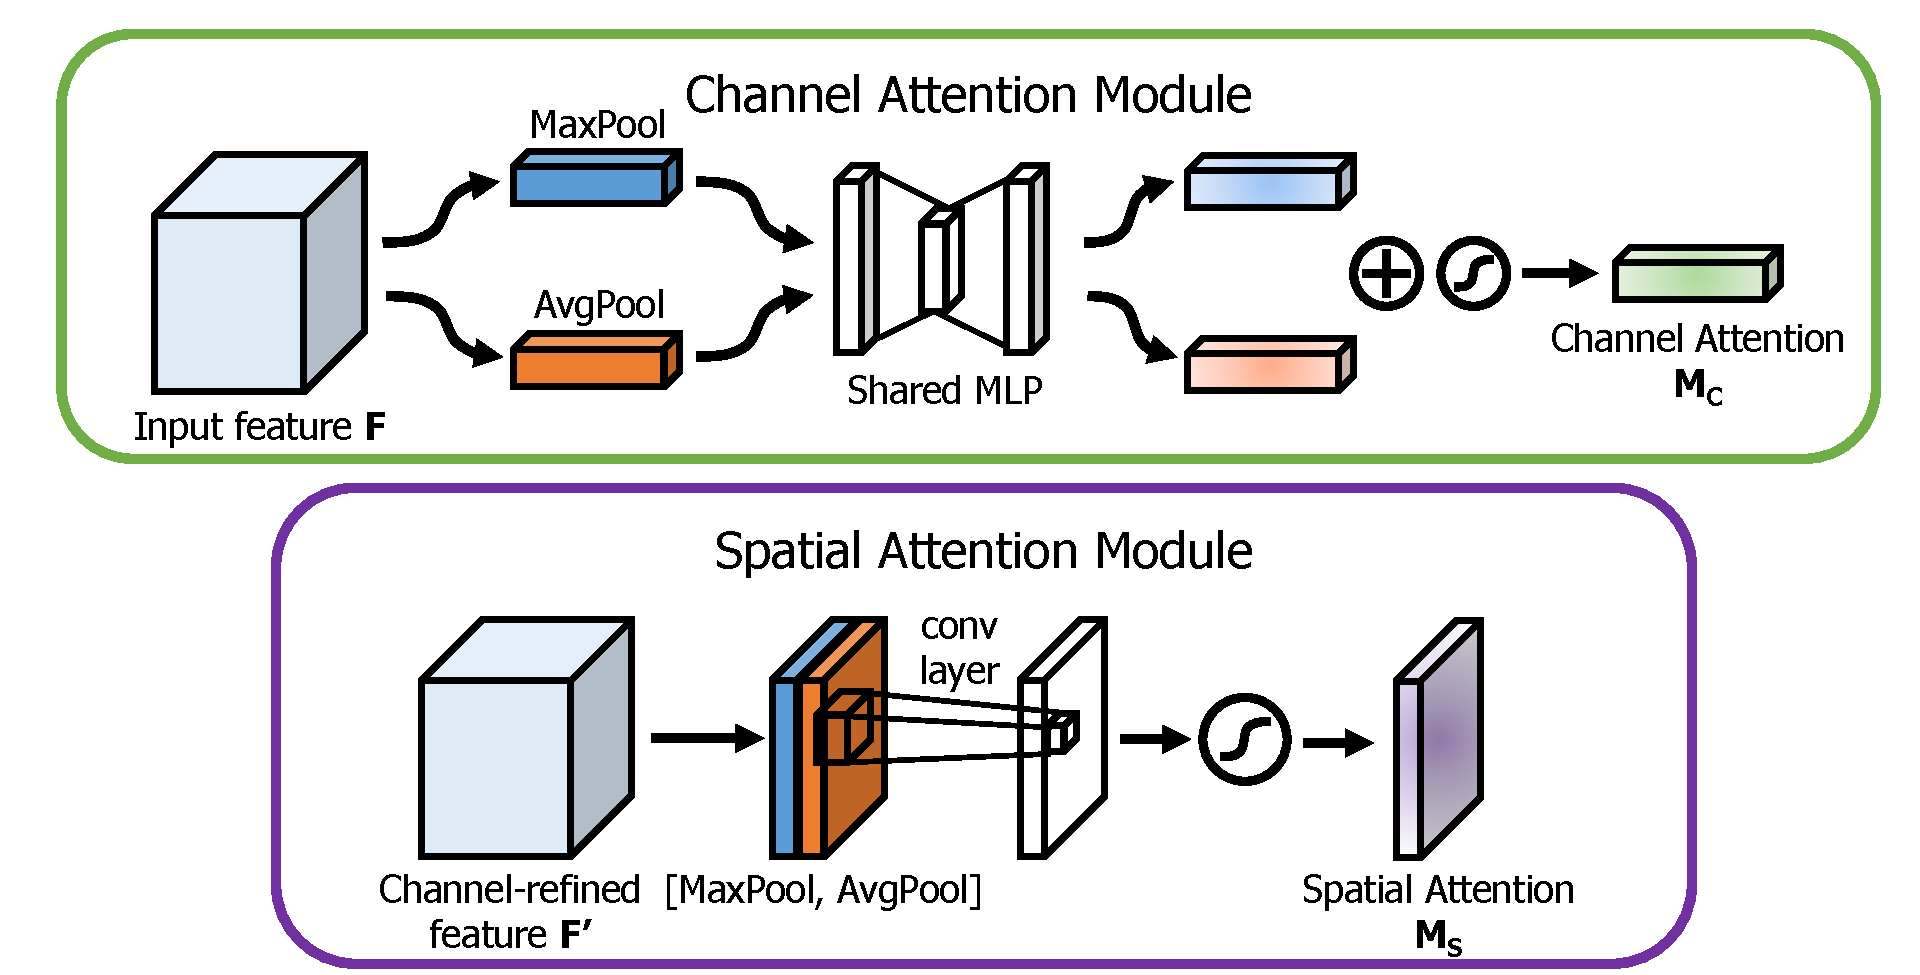
\includegraphics[width=0.6\textwidth]{CBAM-Block.pdf}
    \caption{CBAM模块结构\cite{woo2018cbam}}
    \label{fig:CBAM-Block}
  \end{figure}

具体而言,在通道注意力模块中,输入特征图分别进行空间维度上的全局最大池化和全局平均池化,再将得到的统计值分别通过一个共享权重的全连接层,最后经过逐点加和与非线性变换得到通道注意力权重,用于输入特征图的加权。空间注意力模块的输入是经过通道注意力加权的特征图,首先在通道维度上进行全局最大池化和平均池化,再将得到的统计值在通道维度进行拼接,最后经过卷积降维与非线性变换得到空间注意力权重,与特征图加权后得到最终结果。CBAM的模块结构如图~\ref{fig:CBAM-Block}~所示。

scSE同样结合了通道注意力机制与空间注意力机制,基于SENet提出了一种通道注意力模块(Channel Squeeze-and-Excitation,cSE)和一种空间注意力模块(Spatial Squeeze-and-Excitation,sSE),其结构如图~\ref{fig:scSE}~所示,不同于CBAM,scSE的两个子模块并行处理原始输入,分别在空间维度和通道维度对原始输入进行加权,最后再进行特征图的融合。具体而言,cSE模块中,原始输入依次经过了空间维度的全局平均池化,通道维度的卷积降维与升维,以及非线性变换,以得到通道注意力权重。sSE模块中,直接通过深度卷积在通道维度进行降维,再经过非线性变换以得到空间注意力权重。
\begin{figure}
    \centering
    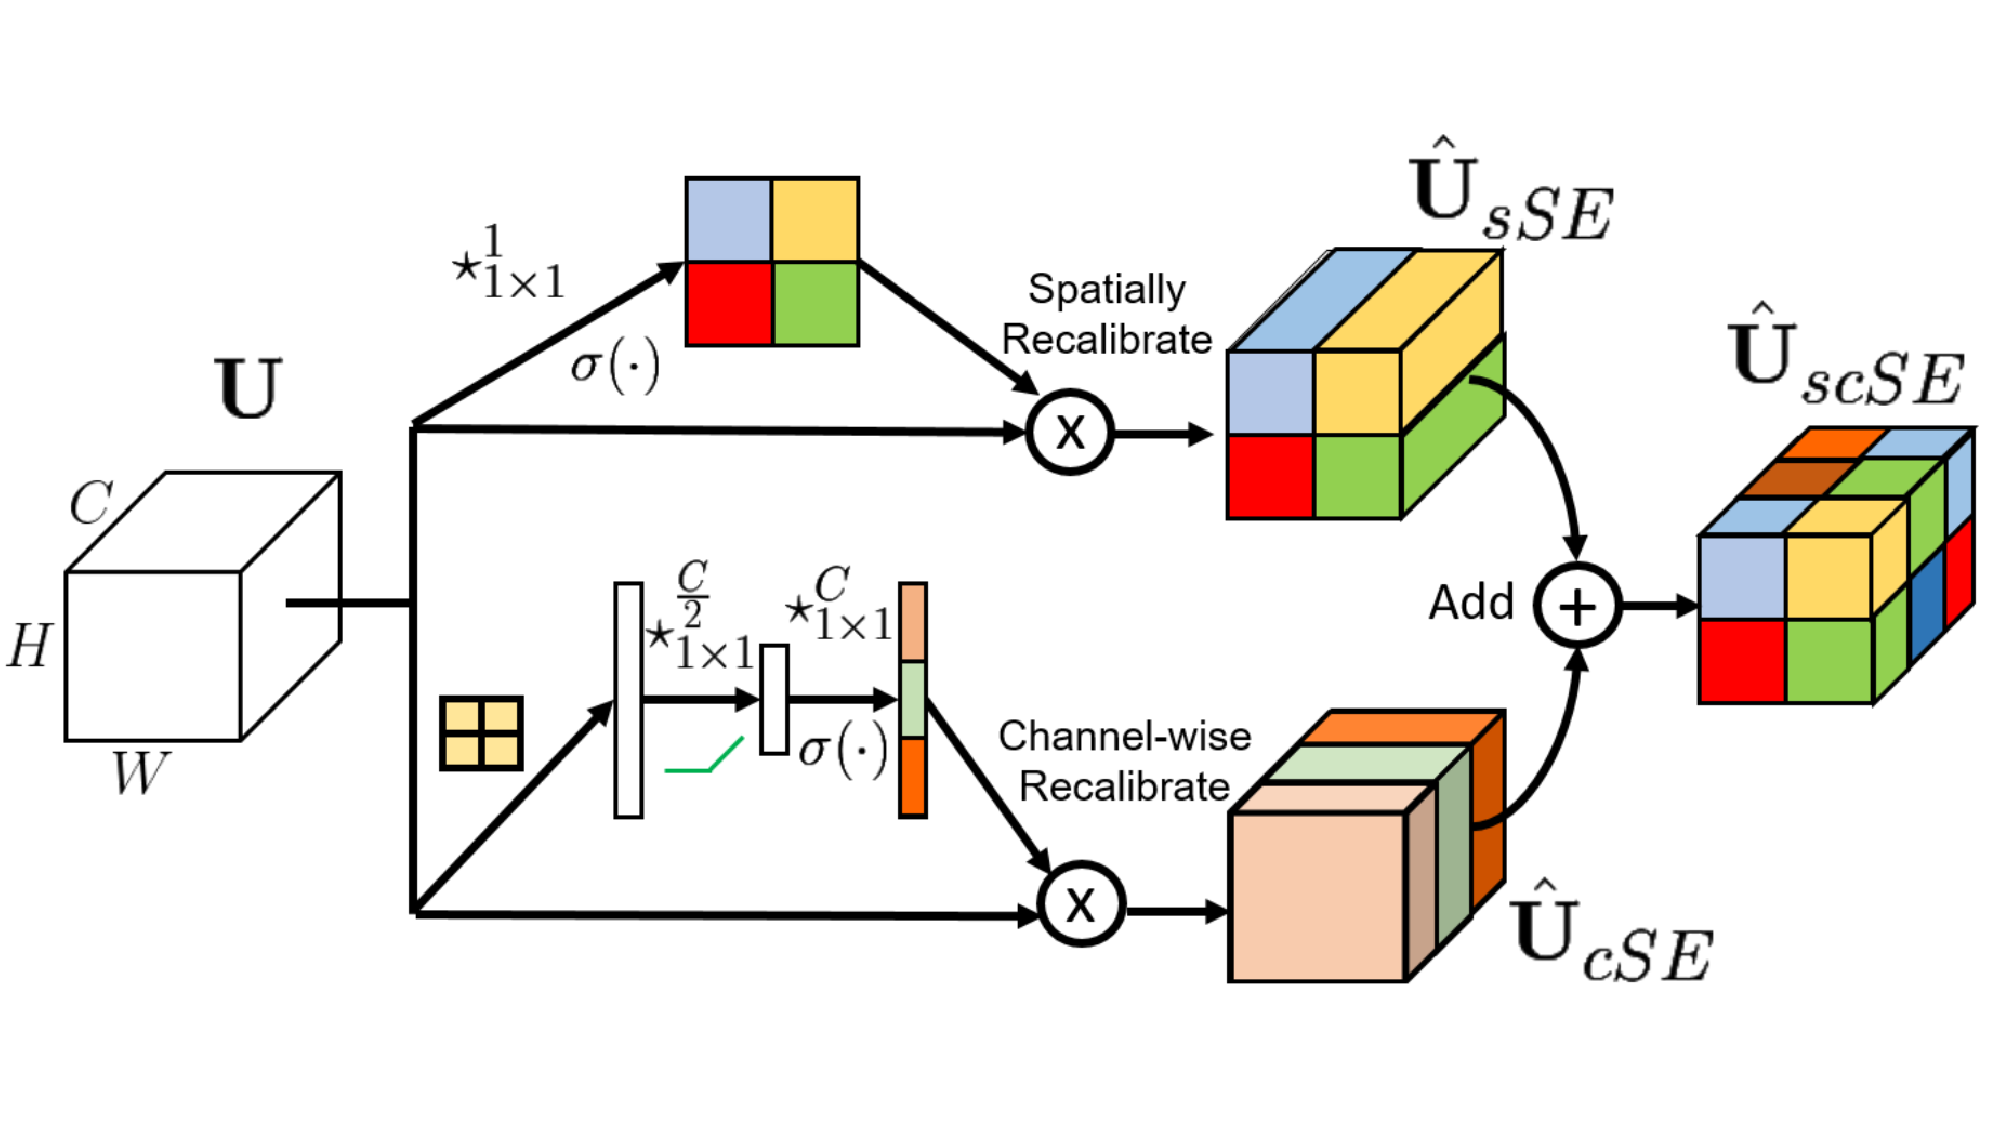
\includegraphics[width=0.6\textwidth]{scSE.pdf}
    \caption{scSE结构\cite{roy2018concurrent}}
    \label{fig:scSE}
\end{figure}

注意力机制通过动态分配权重,使得模型能够聚焦于输入数据中的关键信息,削弱噪声的影响,混合注意力机制则结合了多种注意力机制的优点,从而能够更全面地捕获和整合不同维度的数据特征,并在许多情况下展现出优于单一注意力机制的性能。因此,论文将升维处理后的EEG信号视作具有深度信息的图像数据,采用结合了深度注意力和空间注意力的混合注意力机制对BaseNet进行改进。

CBAM模块和scSE模块均为轻量级注意力模块,且均兼顾深度注意力和空间注意力,但scSE模块在参数数量上更具优势。与此同时,文献\cite{roy2018concurrent}研究发现scSE模块在语义分割任务上表现出色,特别是在与EEG信号拥有相似生理特性的医学图像的分割任务,其性能优于CBAM模块。基于以上理由,论文选择基于scSE模块进行改进,提出了一种新的注意力机制svSE(Separate Variance-Informed Spatial and Channel Squeeze-and-Excitation)模块,其结构如图~\ref{fig:svSE}~所示。
\begin{figure}
    \centering
    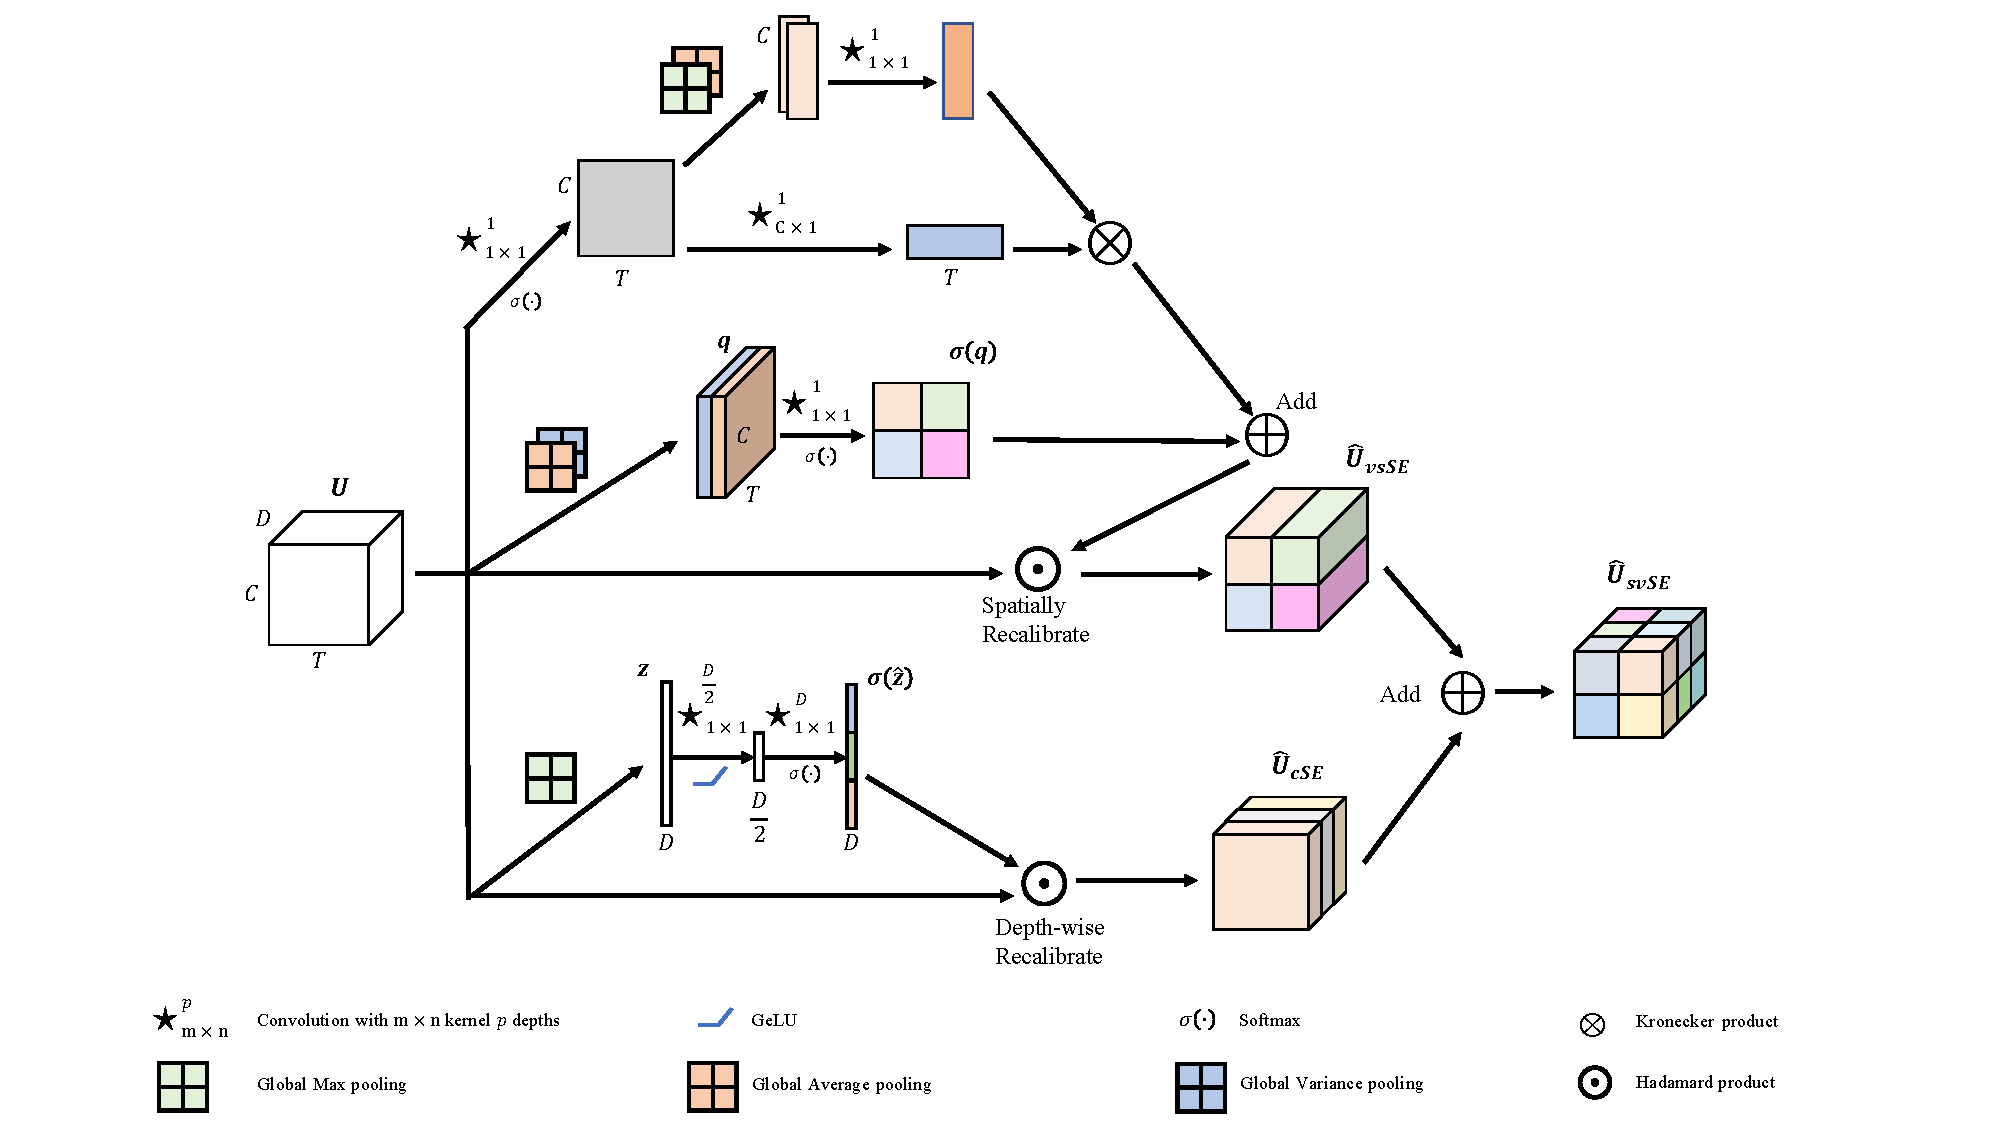
\includegraphics[width=\textwidth]{svSE.pdf}
    \caption{svSE结构}
    \label{fig:svSE}
\end{figure}

针对cSE模块,采用全局最大池化取代全局平均池化操作,用以突出显著特征,得到权重图\(Att_c \in \mathbb{R}^{D \times 1 \times 1}\)。针对sSE模块,论文提出两种方式进行改进,并将两种方式所得的权重相结合以获取最终的输出:

(1) 由CBAM模块的多维全局池化思想以及FBCNet模型的方差层设计\cite{mane2021fbcnet}得到启发,对于输入\(X \in \mathbb{R}^{D \times C \times T}\),采用深度维度上的全局平均池化和全局方差计算操作代替原模块中的压缩操作,得到\(X_{pool} \in \mathbb{R}^{2 \times C \times T}\),随后通过\(1\times1\)卷积对特征图在深度维度进行聚合,得到的权重图\(Att_v \in \mathbb{R}^{1 \times C \times T}\),更好地表征EEG信号特性;

(2) 考虑EEG信号中的时空权重低相关性,即空间特征权重代表电极重要程度,时间特征权重代表采样点重要程度,分两个维度提取特征,获取轴向注意力。对于输入\(X \in \mathbb{R}^{D \times C \times T}\),在空间维度,首先使用\(1\times1\)卷积进行深度压缩操作获得\(X_{sf} \in \mathbb{R}^{1 \times C \times T}\),随后通过时间维度上的平均池化和最大池化得到两个特征图,获得\(X_{spool} \in \mathbb{R}^{2 \times C \times 1}\),通过\(1\times1\)卷积对这两个特征图进行融合,得到\(X_s \in \mathbb{R}^{1 \times C \times 1}\)。对于时间维度,进行空间维度上的卷积操作,以得到时序权重\(X_t \in \mathbb{R}^{1 \times 1 \times T}\)。最后,将空间权重与时序权重以克罗内克积(Kronecker)的方式相乘,恢复维度,得到最终的权重图\(Att_s \in \mathbb{R}^{1 \times C \times T}\)。

其中,\(D\)为输入的深度,\(C\)为空间(通道),\(T\)为时间。此外,使用Softmax激活函数替换Sigmoid激活函数,旨在更好地利用全局信息。由此,整个svSE模块的公式如公式~\ref{eq:svse}~所示,其中,\(\oplus\)为逐元素相加,\(\odot\)为逐元素相乘,\(X_{svSE}\)为加权后的输出。
\begin{equation}\label{eq:svse}
    \begin{aligned}
        &Att_{vs}=Att_v \oplus Att_s \\
        &X_1=Expand(Att_{vs}) \odot X \\
        &X_2=Expand(Att_c) \odot X \\
        &X_{svSE}=X_1 \oplus X_2
    \end{aligned}
\end{equation}

\section{基于LSTM和全局自注意力的分类网络LS-Net}

卷积神经网络倾向于模拟人类视觉系统,卷积层具有局部感受野,能够出色地捕获信号中的局部时空特征,但对于那些跨越较长时间跨度和空间分布的复杂交互信息,其建模能力受限。EEG信号作为随时间变化的信号,具有时间序列属性,长短期记忆网络能够捕获时间域的长期依赖,适合处理序列数据,但缺乏对空间信息进行提取的能力。为此,论文选择LSTM结合全局自注意力的方式,为模型加入时空全局信息。

\subsection{全局自注意力SCoT}

LSTM能够一定程度上捕获序列数据的长期依赖关系,但EEG信号在具有长距离时间依赖的同时具有全局空间特性,使得LSTM无法充分挖掘并整合全局时空域的依赖信息。因此,论文基于Non-local\cite{wang2018non}和Contextual Transformer(CoT)\cite{li2022contextual}这两种全局自注意力机制进行改进,针对EEG信号的特点提出了SCoT(Separate Contextual Transformer)模块,旨在更完整地捕捉EEG信号在时空域内的全局依赖关系,从而增强模型的全局建模能力。
\begin{figure}[h]
    \centering
    \begin{subfigure}{0.4\textwidth}
      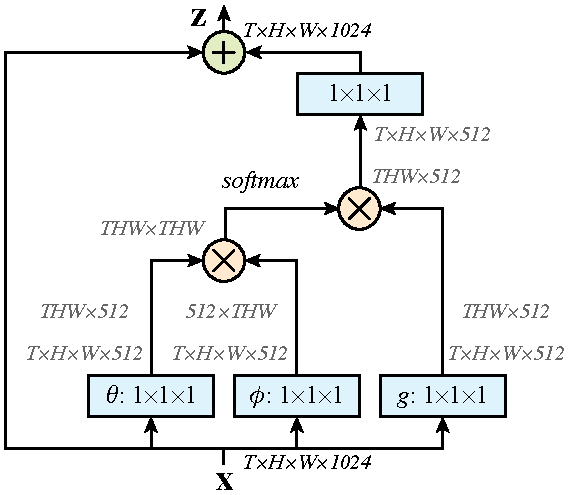
\includegraphics[width=\linewidth]{non-local.pdf}
      \caption{Non-local结构\cite{wang2018non}}
      \label{fig:non-local}
    \end{subfigure}\qquad
    \begin{subfigure}{0.4\textwidth}
      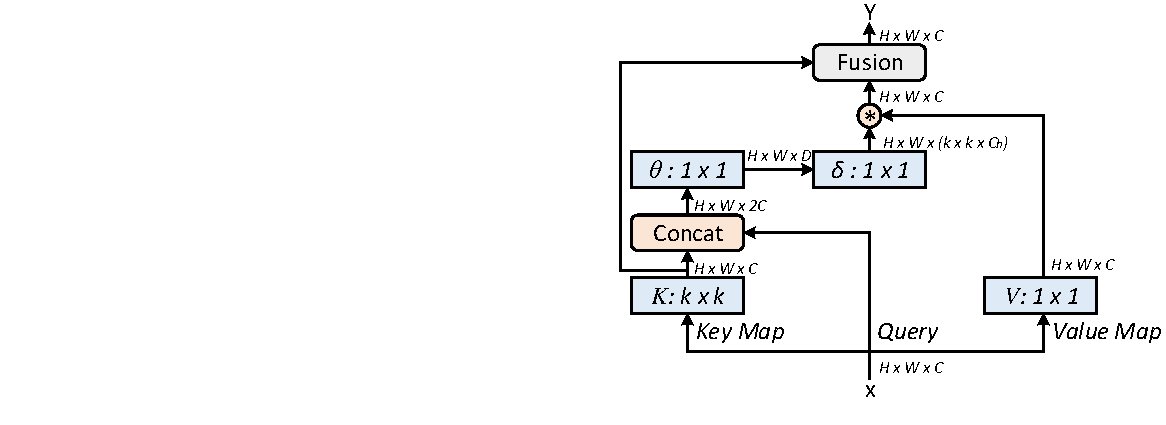
\includegraphics[width=\linewidth]{cot.pdf}
      \caption{CoT结构\cite{li2022contextual}}
      \label{fig:cot}
    \end{subfigure}
    \caption{两种全局自注意力}
    \label{fig:self}
\end{figure}

(1) Non-local

Non-local是将自注意力\cite{vaswani2017attention}应用于计算机视觉领域的一项经典模型,能够捕捉特征图中任意两个位置之间的依赖关系,其结构如图~\ref{fig:non-local}~所示。对于输入\(X \in \mathbb{R}^{C \times H \times W}\),首先通过三个\(1\times1\)卷积将通道数量由\(C\)压缩为\(\frac{C}{2}\),分别得到代表查询(Query)、键(Key)和值(Value)矩阵的三个特征图\(X_\theta\)、\(X_\phi\)和\(X_g\)。随后对\(X_\theta\)、\(X_\phi\)、\(X_g\)进行展平(Flatten),并通过点积操作计算\(X_\theta\)与\(X_\phi\)的相似度矩阵\(S\),该矩阵代表输入特征图中各个位置之间的联系。接着,使用Softmax函数对相似度矩阵\(S\)进行归一化,使得其转化为概率分布,并与值矩阵\(X_g\)相乘,得到结果矩阵\(Y \in \mathbb{R}^{\frac{C}{2} \times H \times W}\),最后,通过\(1\times1\)卷积恢复\(Y\)的维度至与\(X\)相同,以逐元素相加的方式得到加权后的结果。Non-local通过直接计算两个位置之间的远程依赖关系,能够获取全局自注意力,但在数据量较大的情况下,存在计算量偏大的问题。

(2) CoT

CoT考虑到Non-local忽略了相邻键上下文信息的问题,提出了一种将上下文信息挖掘能力集成入自注意力机制中的方式,其结构如图~\ref{fig:cot}~所示。对于输入\(X \in \mathbb{R}^{C \times H \times W}\),CoT的改动主要在于使用\(3\times3\)卷积获取特征图的静态上下文信息,将其作为键矩阵\(K\),同时,通过\(1\times1\)卷积获取到值矩阵\(V\),直接获取了查询矩阵\(Q\),然后对\(K\)和\(Q\)进行深度维度的聚合,并通过两个连续的\(1\times1\)卷积获取注意力权重图\(A\),通过注意力权重图\(A\)和值矩阵\(V\)相乘获取特征图的动态上下文信息,最后将静态上下文信息和动态上下文信息进行了融合。

对于运动想象MI-EEG分类任务来说,问题在于EEG信号的特性:EEG信号的时域和空域上具有较低的局部相关性;在空域上,尽管相邻的电极具有空间相关性,但在EEG原始输入中,相邻的电极未必排列为相邻的通道,因此,在端到端网络的情况下,空域内具有较低的局部相关性;在时域上,EEG信号具有局部相关性,即相邻的采样点往往蕴含相似的信息。因此,Non-local模块和CoT模块无法直接迁移至运动想象MI-EEG分类任务中:Non-local模块能够计算任意两个位置之间的远程依赖关系,但在较大的数据量下,其计算代价高昂;而CoT模块则是基于图像数据的局部相关性,将局部上下文信息引入了自注意力机制中,并通过卷积操作减少了计算量。论文借鉴Non-local和CoT的思想,提出了SCoT模块。

综合考量EEG信号的时空特性与Non-local、CoT各自的特点,论文提出的SCoT注意力模块采取了时空域分步计算全局自注意力的策略,具体来说,针对空域中局部相关性较弱且数据规模有限的情况,对Non-local模块进行改良以适应空间自注意力计算;而对于具有强局部相关性且数据规模较大的时域信息,基于CoT进行改进以计算时间自注意力。SCoT的结构如图~\ref{fig:gsa}~所示。
\begin{figure}
    \centering
    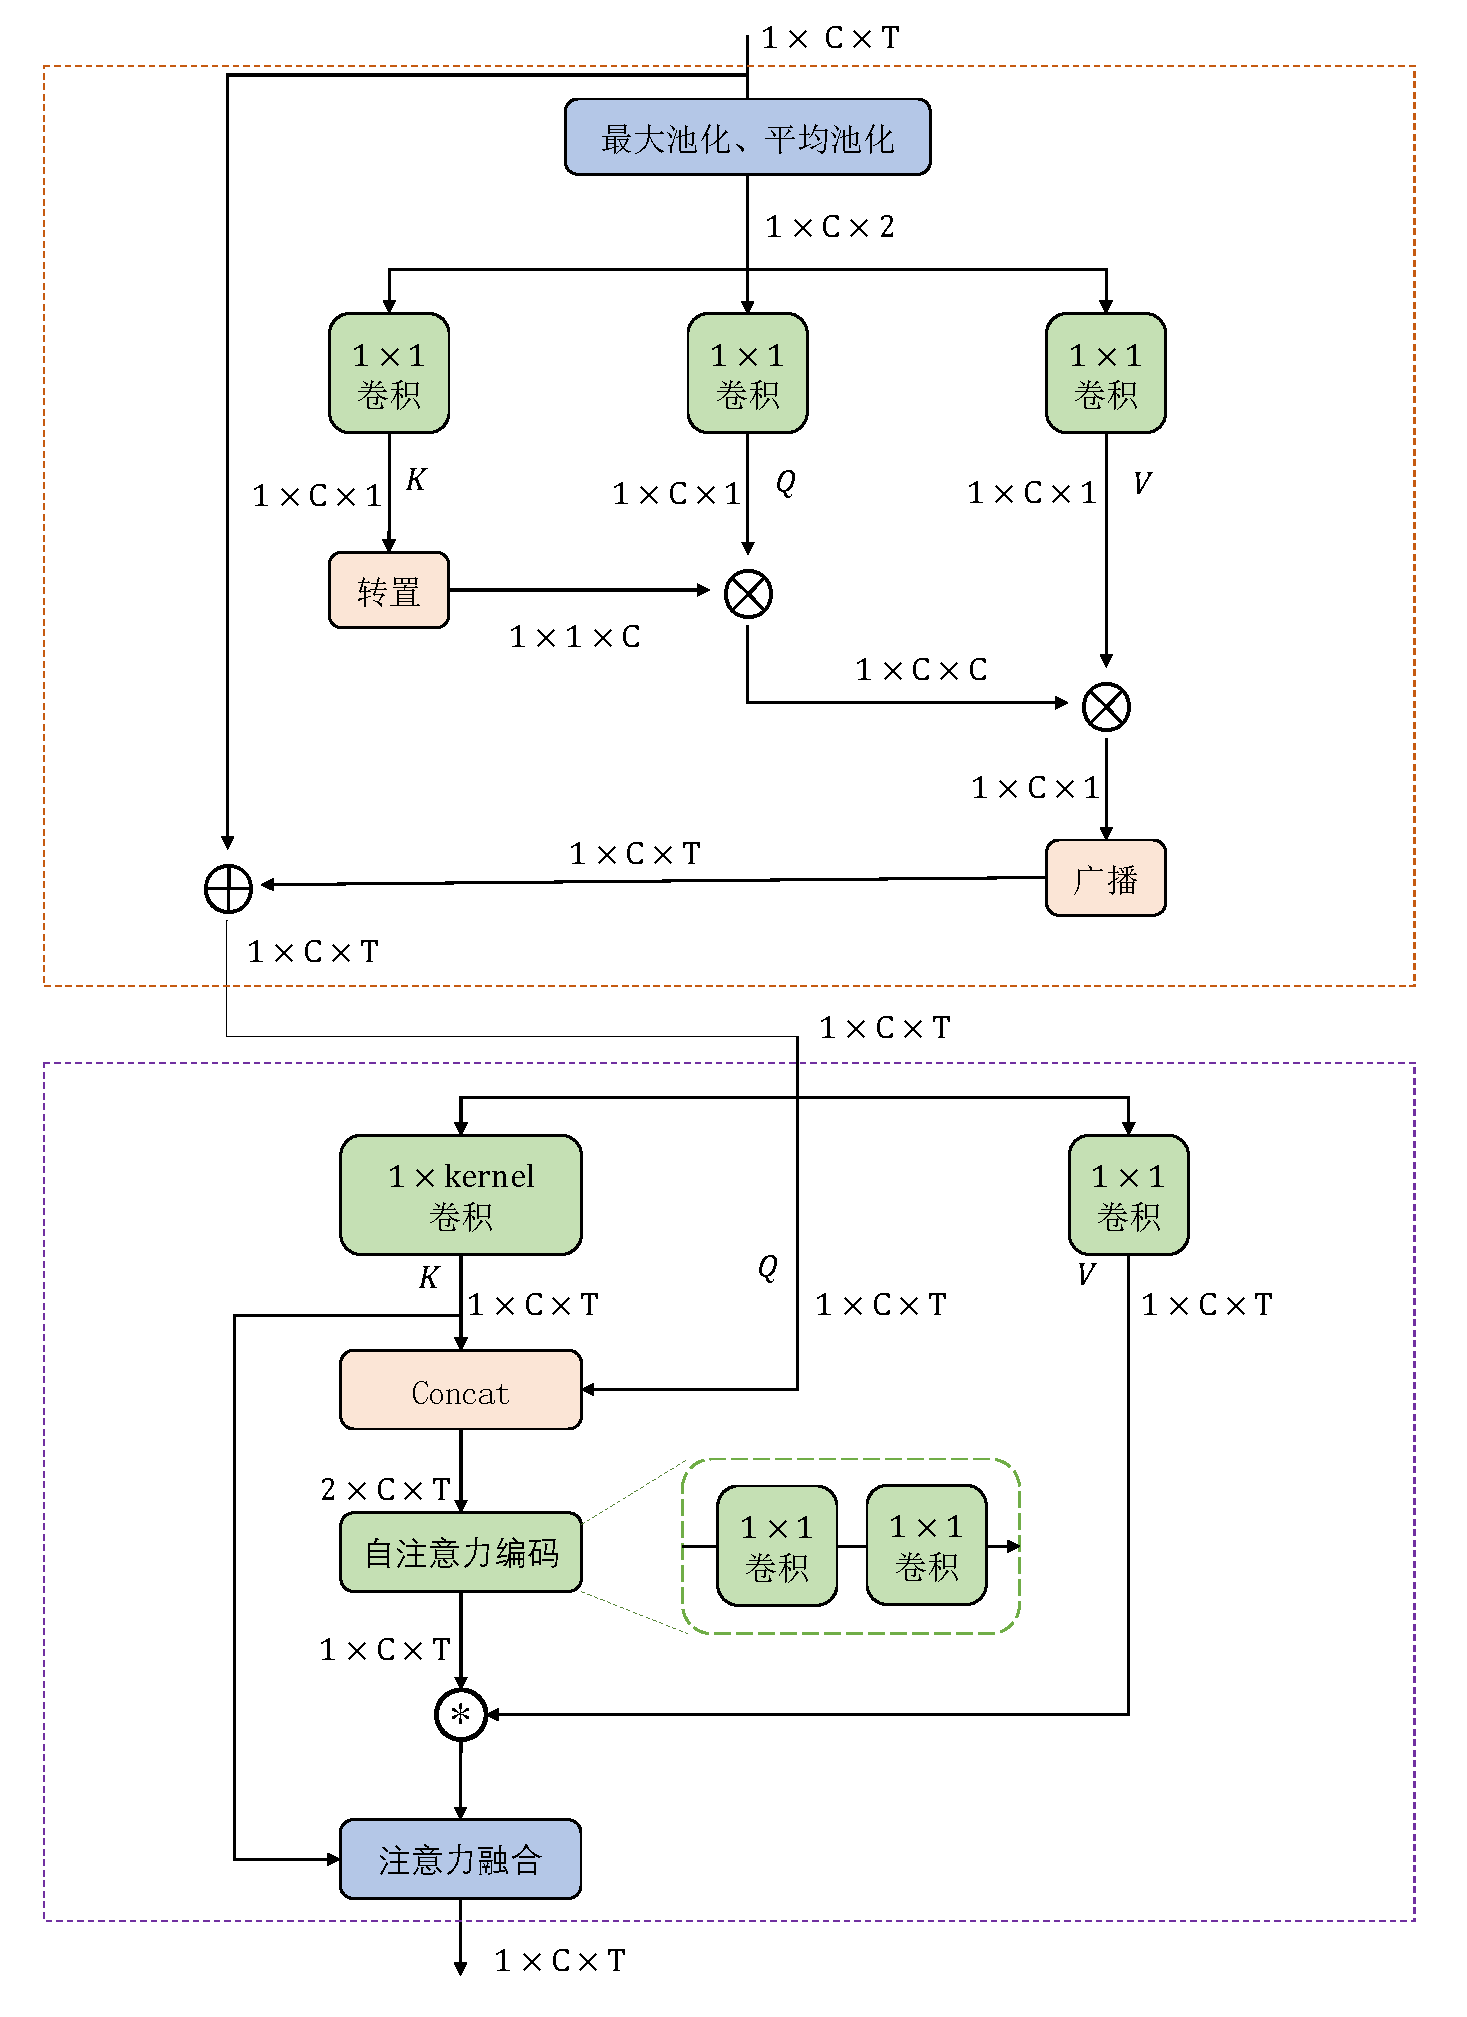
\includegraphics[width=0.5\textwidth]{gsa.pdf}
    \caption{SCoT结构}
    \label{fig:gsa}
\end{figure}

SCoT分两个过程计算EEG信号的全局时空注意力,首先计算空域上的空间自注意力,使用空间自注意力对输入进行加权后,再基于加权数据计算时空域自注意力。空间自注意力能够为重要的电极(通道)分配更多的注意力,在局部相关性较弱的情况下突出不同通道的相对重要性。时空域自注意力能够充分利用时间序列数据中的局部相关性,以及已经由空间自注意力加权强化过的空间特征信息,从而更加精细而全面地捕获EEG信号中的全局时空依赖关系。此外,两个过程的计算也有利于降低计算的复杂度。

SCoT模块计算注意力的整体流程如公式~\ref{eq:scot}~所示,其中,\(X\)为EEG信号输入,\(C\)为通道,\(T\)为时间,\(Att_s\)为空间自注意力模块,\(Att_{st}\)为时空自注意力模块。
\begin{equation}
    SCoT(X)=Att_{st}(Att_s(X)), \; X \in \mathbb{R}^{1 \times C \times T}
    \label{eq:scot}
\end{equation}

在空间自注意力模块中,首先进行混合池化操作,对输入进行转换:
\begin{equation}
    X'=Concat[MaxPool(X),AvgPool(X)],\;X' \in \mathbb{R}^{2 \times C \times T}
    \label{eq:scots1}
\end{equation}
EEG信号具有低信噪比的特性,混杂了大量的噪声和干扰成分,通过结合最大池化操作和平均池化这两种操作,能够能够在最大程度保留EEG信号中关键特征的同时,对噪声起到一定的抑制作用,从而在不同的特征信息之间取得平衡。在取得池化表示\(X'\)后,通过公式获得键(Key)、查询(Query)、值(Value)矩阵\(K\)、\(Q\)和\(V\),其中,\(W_K,\,W_Q,\,W_V\)分别是对应的权重参数,通过\(1\times1\)卷积获得。
\begin{equation}\label{eq:scots2}
    K=X'W_K,\;Q=X'W_Q,\;V=X'W_V
\end{equation}
随后,将\(K\)经过转置后与\(Q\)相乘,提取其相似性特征,并使用Softmax进行归一化,得到权重矩阵\(A\),得到的计算过程如公式~\ref{eq:scots3}所示,其中,\(\bigotimes\)代表克罗内克积:
\begin{equation}\label{eq:scots3}
    A=Softmax(Q \bigotimes K^T),\;A \in \mathbb{R}^{1 \times C \times C}
\end{equation}
\(A\)随后与值矩阵\(V\)相乘,实现对特征图的加权,并通过广播方式扩展到与输入特征图相同的尺寸,与输入特征图\(X\)加和后得到空间自注意力的输出,计算过程如公式~\ref{eq:scots4}~所示。
\begin{equation}\label{eq:scots4}
    Att_s(X)=X+Expand(A \bigotimes V)
\end{equation}

空间自注意力的输出被作为时空域自注意力模块的输入,以在时空域中利用经过强化的空间特征。首先通过\(1 \times kernel\)卷积提取时间域上的局部上下文特征,使得生成的键矩阵\(K\)具有输入特征图的静态上下文信息,对查询矩阵\(Q\)不做变换,使用\(1\times1\)矩阵获取值矩阵\(V\)。对于经过空间自注意力加权后的输出\(Y  \in \mathbb{R}^{1 \times C \times T}\),三个矩阵的计算过程如公式~\ref{eq:scotst1}~所示,\(W_K,\,W_V\)分别是键矩阵和值矩阵对应的权重参数,在计算上,使用卷积进行获取,其过程如公式~\ref{eq:scotst2}~所示。
\begin{equation}\label{eq:scotst1}
    K=YW_K,\;Q=Y,\;V=YW_V
\end{equation}
\begin{equation}\label{eq:scotst2}
    W_K=Conv_{1 \times kernel}(Y),\;W_V=Conv_{1 \times 1}(Y),\;kernel=\left \lfloor \frac{sfreq}{4} \right \rfloor 
\end{equation}
其中,\(kernel\)的值取决于采样率\(sfreq\),在此设定为\(\left \lfloor \frac{sfreq}{4} \right \rfloor\),是为了捕获4Hz以上的频率信号。

随后,\(K\)和\(Q\)在深度维度进行聚合,提取其相似度特征,并于\(V\)矩阵进行融合,获取特征图的动态上下文信息\(L\),其计算过程如公式\ref{eq:scotst3}~所示:
\begin{equation}\label{eq:scotst3}
    L=Fusion(V ,\, (Conv_{1 \times 1}(Conv_{1 \times 1}(Concat[K,Q])))),\;L \in \mathbb{R}^{1 \times C \times T}
\end{equation}
其中,\(\odot\)表示逐元素相乘的Hadamard乘法。通过两个\(1 \times 1\)卷积进行自注意力编码运算,学习动态多头注意力矩阵。\(Fusion\)为局部矩阵乘法运算,用于度量局部网格中每个query与相应key之间的成对关系,在计算上,公式表示了\(Fusion\)运算的集合,在时间域和空间域分别使用轴向卷积进行了局部矩阵乘法运算,随后进行了\(BN\)批量归一化和\(Softmax\)归一化。
\begin{equation}\label{eq:scotst4}
    Fusion=Conv_{channels \times 1}+Conv_{1 \times kernel} + BN + Softmax
\end{equation}

最后,将输入特征\(Y\)与\(L\)进行融合,得到时空域自注意力模块的输出\(Att_{st}\),如公式~\ref{eq:scotst4}~所示。其中,\(\odot\)表示逐元素相乘的Hadamard乘法。融合方式参考了Transformer的残差连接思想,将\(Y\)与\(L\)经过Concat聚合之后由卷积进行融合,从而实现对特征的校准,最后,通过逐元素相乘得到校准后的加权输出。计算期间,对数据进行了多项变形(Reshape)操作。
\begin{equation}\label{eq:scotst5}
    Att_{st}=Softmax(Conv_{1 \times 1}(AvgPool(Concat[Y,L]))) \odot Y
\end{equation}

对运动想象脑电图分类任务来说,传统的全局自注意力机制忽视了EEG信号时域与空域的低局部相关性,导致网络无法很好对重要数据进行关注。SCoT通过两个过程进行全局时空注意力的提取,对EEG信号具有更好的适应性,同时降低了计算的复杂度。空间全局自注意力能够突出不同通道数据的重要性,为时空域的全局自注意力提供先验信息,时空域的全局自注意力利用时间域的局部上下文信息和轴向卷积,将输入特征图的静态上下文和动态上下文进行结合,能够增强输出特征图的表征能力。

\subsection{基于LSTM和SCoT的分类网络}

长短期记忆网络(Long Short-Term Memory,LSTM)属于循环神经网络,能够利用当前时间步及其之前的信息,并且解决了RNN在处理长期依赖问题时存在的梯度消失和梯度爆炸问题。LSTM通过单元状态存储和更新信息,使得模型能够记住历史信息,并且有选择地进行遗忘或者更新;通过门控机制(输入门、遗忘门、输出门),LSTM能够对信息的流动进行有效的控制,从而保留和传递长距离信息,提升对长期依赖关系的建模能力。考虑到LSTM具有出色的对时序数据进行建模的能力,论文选择使用LSTM来获取EEG信号中的时序长期依赖信息。

LSTM用于处理形状为\((sequence\_length,\, batch\_size,\, input\_size)\)的三维序列数据,其中\(sequence\_length\)为序列的长度,\(batch\_size\)为批量处理的样本数量,\(input\_size\)为每个时间步的特征维度。其输出同样是三维序列数据,形状与输入序列类似,具体为\((sequence\_length,\,batch\_size,\, hidden\_size)\),其中,\(hidden\_size\)为LSTM内部的隐藏维度。LSTM由一系列元胞连接而成,这些元胞按时间顺序逐个处理输入序列,在每一个时间步内,LSTM元胞进行以下操作:计算当前时间步的输入允许计入单元状态的程度;判断单元状态中应当被丢弃的信息;计算候选单元状态;更新单元状态;生成当前时间步的隐藏状态,以及将隐藏状态传递给下一个时间步或输出。

EEG信号是使用脑电采集设备采集的大脑在一段时间内的电压变化,天然具有时序属性,原始EEG信号为时间和通道的二维数据,其中,时间维度可以对应LSTM输入的序列长度,通道维度可以对应LSTM输入的特征维度。由此,可以将EEG信号以\((time\_samples,\, batch\_size,\, channels)\)的形式与LSTM的输入对齐,即将通道维度视为对应时间步(采样点)上数据所具有的特征。

虽然LSTM通过其内部的单元状态和门控结构缓解了RNN中存在的长期依赖的问题,但在处理较长的时间序列数据时,其性能仍存在局限性。LSTM在遍历时间序列的过程中,对每个时间步的输入信息均采用统一的方式通过隐藏状态进行累积和更新,并不具备针对当前任务为各个时间步的输入赋予不同重要性的能力。因此,有必要在LSTM模型中引入全局时空注意力机制SCoT模块,使得模型能够动态地对EEG信号中的重要数据进行关注,理解不同位置之间的深层次依赖关系,捕获更为完整的长距离信息,从而获得更为精确和全面的特征表示,提升模型处理EEG信号分类任务时的性能和泛化能力。

LSTM结合SCoT得到的网络结构如图~\ref{fig:ls}~所示,将其称之为LS-Net(LSTM-SCoT Net)。
\begin{figure}
    \centering
    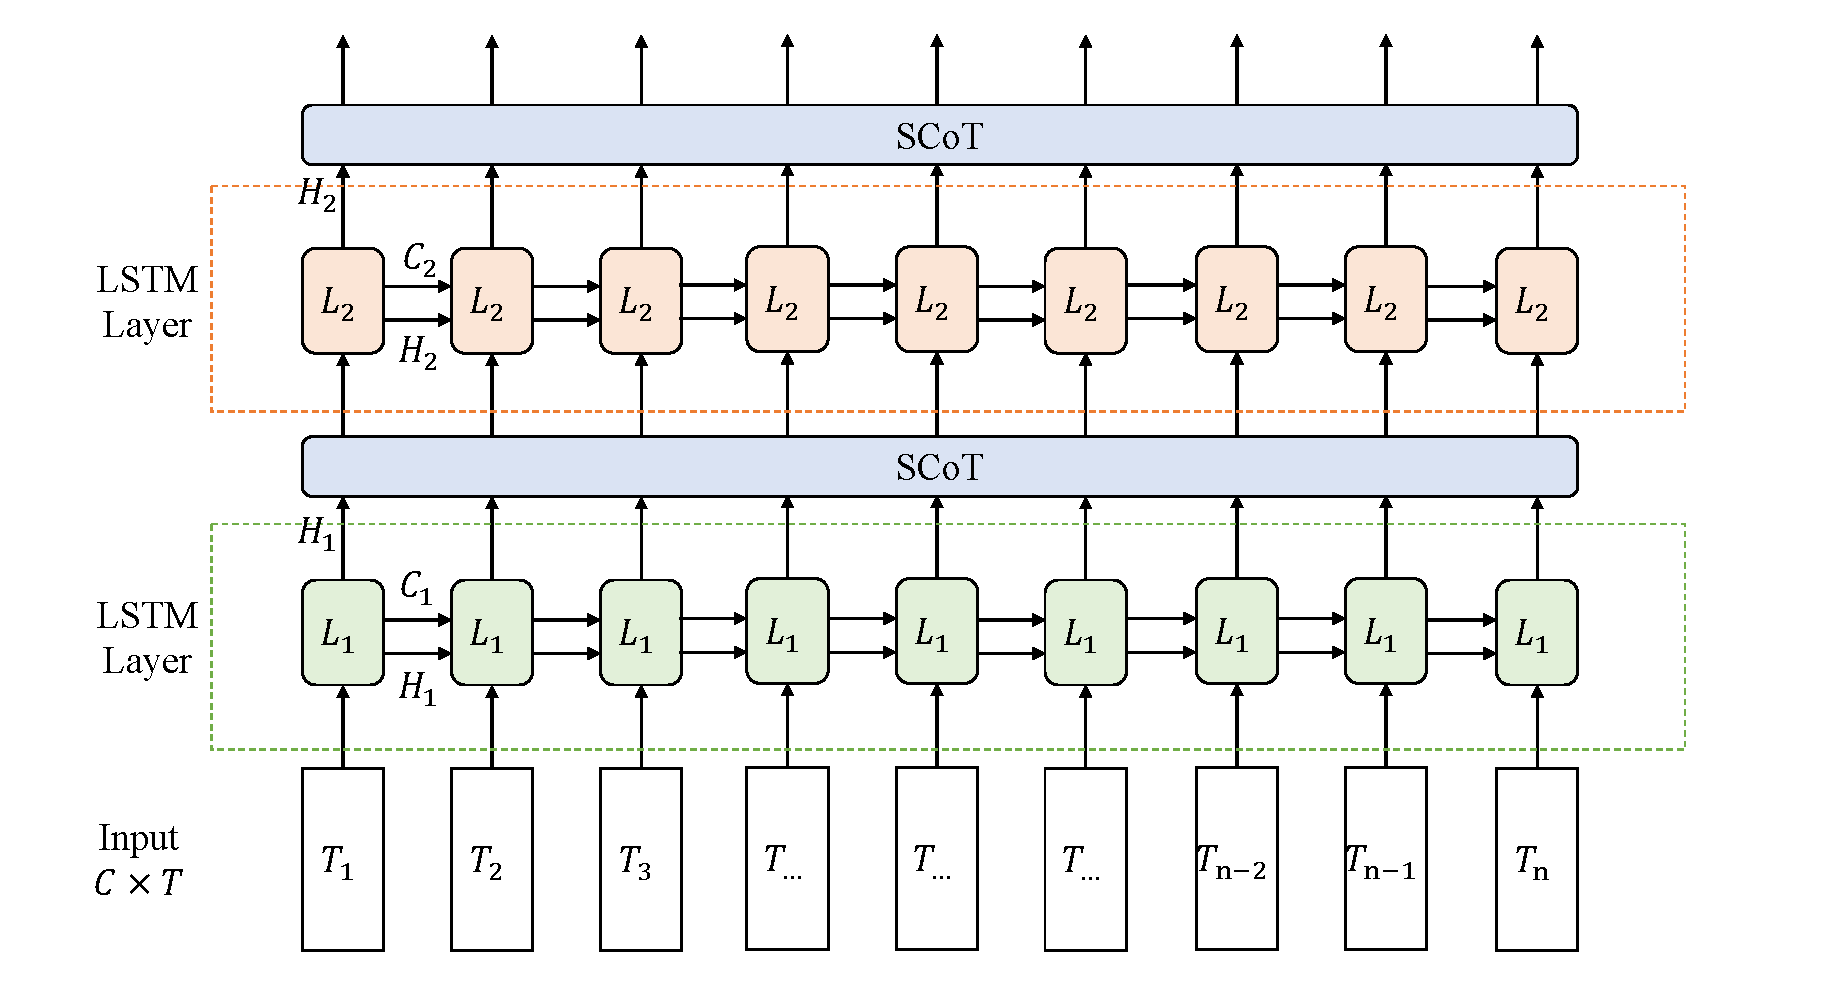
\includegraphics[width=\textwidth]{ls-net.pdf}
    \caption{LS-Net结构}
    \label{fig:ls}
\end{figure}
LS-Net的输入为\(X \in \mathbb{R}^{C \times T}\),其中,\(C\)为通道数量,表示每个时间采样点所具有的特征数,\(T\)为时间,表示表示时间轴上的采样点序列长度。
在处理过程中,LSTM按时间序列递进地对每个采样点进行加工,LSTM的每个层(Layer)的输出结果为\(Y \in \mathbb{R}^{H \times T}\),其中,\(H\)为隐藏层数量。
在经过每个Layer处理后,\(Y\)由SCoT模块计算全局时空自注意力。需要说明的是,尽管\(H\)来自于LSTM的隐藏层维度,但在SCoT模块中,仍然将其视为通道维度特征进行处理,以对来自LSTM输出的特征进行整合,从而提升网络捕捉输入EEG信号全局时空依赖关系的能力。

为了综合LS-Net和DIS-Net的优点,论文选择以并行分支的形式将LS-Net引入DIS-Net网络结构中。这是因为直接以串联形式加入LS-Net可能导致模型仅能捕捉到经过深层卷积获得的特征图的依赖关系,而非充分利用全局信息。并行分支的设计旨在全面利用LS-Net对全局依赖的建模能力,同时避免干扰卷积神经网络本身的局部特征提取功能。

将LS-Net模块引入DIS-Net后获得的新模型命名为HA-FuseNet,其结构如图~\ref{fig:hafuse}~所示。

为了整合DIS-Net与LS-Net所提取的特征信息,将二者获取的特征图在深度维度进行特征聚合。为了确保两个分支的数据能够聚合,需要对数据形状进行适配处理。此外,由于需要使用历史信息,LSTM无法进行并行计算,因此同样需要对于输入LSTM的数据进行一定的处理,以对计算效率进行平衡。

论文设计了C2R-Block和R2C-Block两种模块,用于并行分支间的交互融合。在C2R-Block中,对数据执行时间维度的卷积操作以实现下采样,将原始样本 \(X \in \mathbb{R}^{C \times T}\) 在时间轴上进行压缩,转化为 \(X' \in \mathbb{R}^{C \times T'}\) ,其中, \(C\) 代表通道数(电极数), \(T\) 代表原始时间序列长度,\(T'\)则代表下采样后的时间序列长度。另一方面,在R2C-Block中,采用反卷积技术对LS-Net模块产生的输出进行时间维度上的上采样,使其与DIS-Net分支的数据维度相符。最后,在深度维度对经过上述处理的两类特征进行聚合,从而充分融合卷积神经网络捕获的局部特征信息、长短期记忆网络揭示的时序依赖特性,以及全局自注意力模块发掘的全局时空依赖关系,以期全面提升模型对EEG信号的综合理解与分析能力。

\section{基于GhostNet改进的网络轻量化}

考虑到BCI系统对即时响应具有较高的要求,虽然HA-FuseNet通过轴向卷积和深度可分离卷积削减了一定的模型参数量,但为了追求更加卓越的实时性能表现,仍有进行进一步轻量化的必要。HA-FuseNet模型的参数主要来源于密集连接模块、长短期记忆网络和全局自注意力。针对长短期记忆网络和全局自注意力,论文通过下采样削减了输入数据的规模。与此同时,对于密集连接模块以及其他卷积层,论文进行针对性的轻量化卷积设计,并将在下文中对轻量化卷积模块的设计思路与方案加以阐述。

\subsection{经典轻量级网络结构}

MobileNet\cite{howard2017mobilenets}由Google团队提出,其核心思想在于引入了深度可分离卷积(Depthwise Separable Convolution),通过深度卷积处理单个输入通道,然后使用点积卷积(也称为逐点卷积或\(1 \times 1\)卷积)跨通道整合信息。这种分解大幅减少了计算成本和模型大小,同时保持了较高的精度。

ShuffleNet\cite{ma2018shufflenet}由旷视科技的研究团队所开发,其设计目标在于实现模型计算效率与预测准确性的均衡优化。ShuffleNet将输入特征图均匀划分为两个部分,一部分不经额外计算直接向下传输,另一部分则经历一系列计算后再与前者合并。二者在concatenate操作之后,实施通道混洗操作,从而有效提升模型在轻量化条件下的性能表现。

\begin{figure}
    \centering
    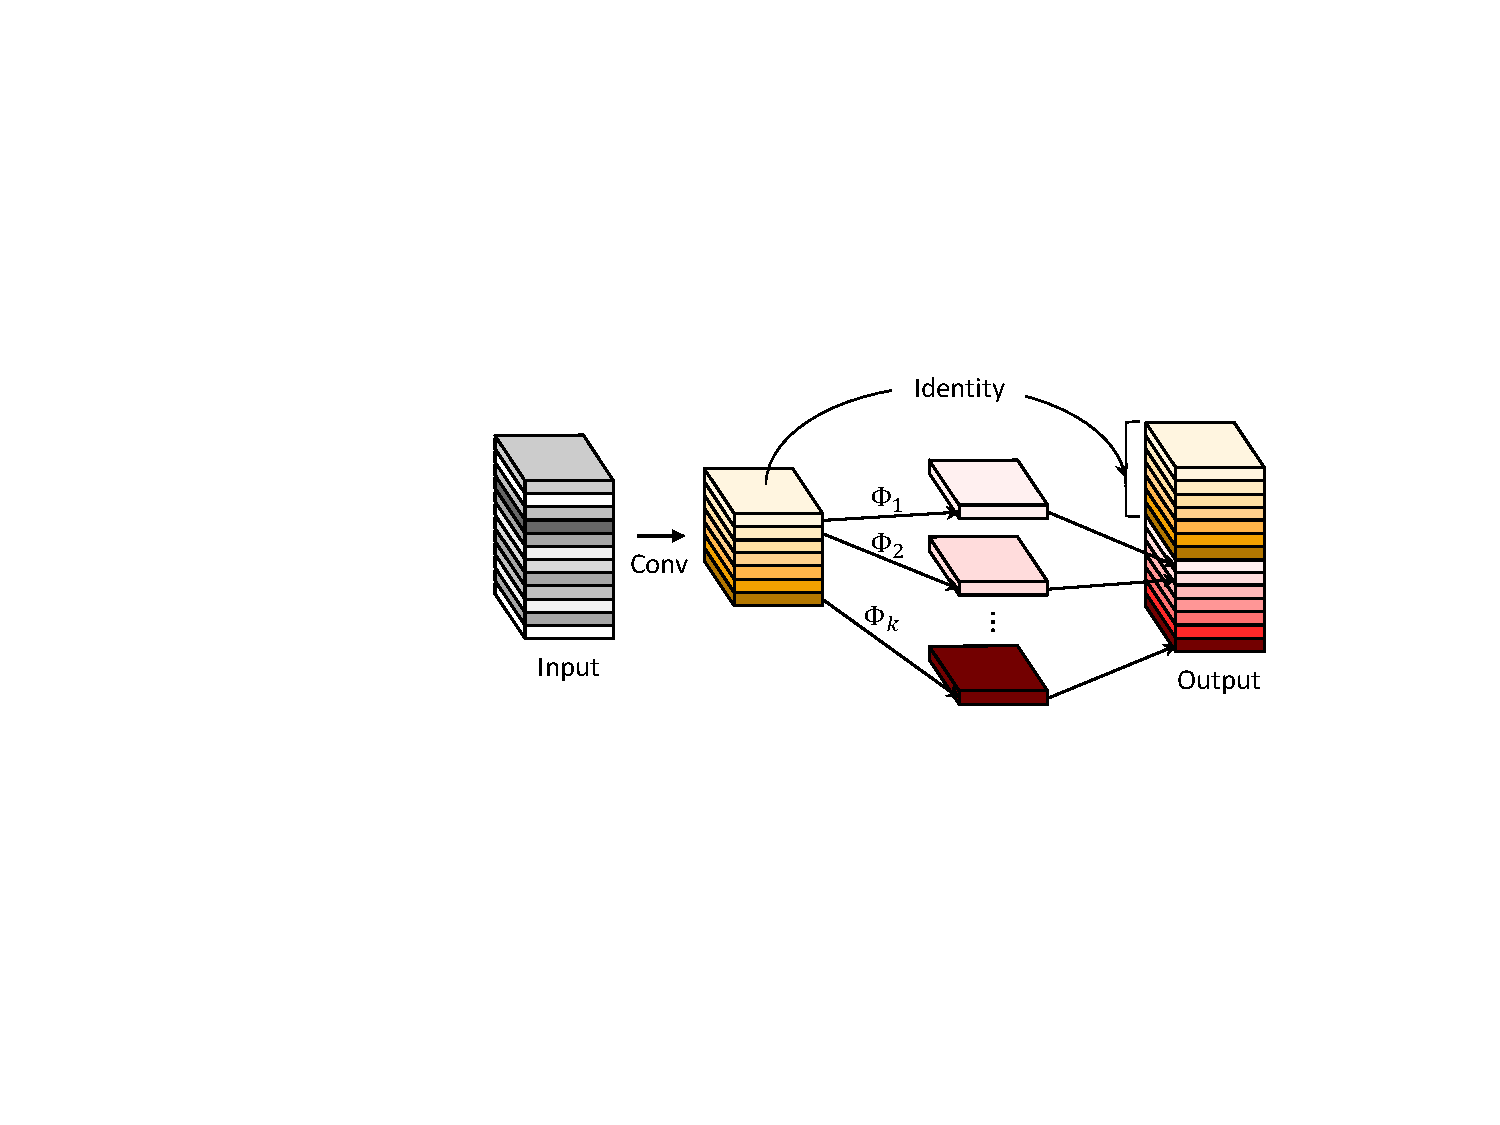
\includegraphics[width=0.6\textwidth]{ghost.pdf}
    \caption{Ghost模块结构\cite{han2020ghostnet}}
    \label{fig:ghost}
\end{figure}
GhostNet\cite{han2020ghostnet}由华为诺亚方舟实验室提出,其核心思想在于提出了幻影模块(Ghost Module),该模块针对深度神经网络中存在的潜在冗余和相关性较高的特征图问题,通过高效的计算策略提炼出“幻影特征图”。研究团队发现,在许多情况下,多个特征图可能蕴含着相似的模式信息,这意味着部分特征图的信息实质上可以从其他特征图中推衍得出,犹如“幻影”。鉴于此,GhostNet摒弃了对每组特征图均采用标准卷积的传统做法,转而采用一种更为经济高效的计算方式去合成这类“幻影特征图”。在具体实施中,首先运用有限数量的标准卷积层提取基础特征图,以此严格控制参数规模,接下来通过对基础特征图施加一组线性变换,高效地生成大量辅助特征图,这些辅助特征图被视为原始特征图的“幻影”。最后,Ghost模块将“幻影特征图”与标准卷积产生的少量核心特征图整合在一起,以有效模拟传统卷积所带来的丰富表征能力,在保持高精度的同时,降低了模型的计算复杂性和参数规模。Ghost模块的结构如图~\ref{fig:ghost}~所示,其中,Identity操作由标准卷积生成的特征图,\(\Phi\) 为廉价线性变换。

\subsection{GhostNet结合MobileNet改进的轻量化卷积模块}

在HA-FuseNet架构中,已经通过轴向卷积削减了一定的模型参数量。因此,本节在现有成果的基础上,主要结合ShuffleNetV2的基础单元和GhostNet所提出的Ghost模块进行了针对性改良。

GhostNet的优势在于其Ghost模块设计,该模块凭借对特征图间内在相似性的有效利用,实现了低成本的特征转换操作,同时,GhostNet中使用了权重参数 \(ratio\),用以控制经由廉价线性转换进行操作的特征图的比例,其中,使用标准卷积的生成的特征图数量为\(D_{out} \times ratio\),其中,\(D_{out}\)为输出特征图数量,使用深度卷积的分支生成的特征图数量为\(D_{out}-D_{out} \times ratio\)。

然而,Ghost模块在运用线性变换与传统卷积相结合的方式来产生新特征图的过程中,尚存在一定的局限性:在深度可分离卷积的实现上,Ghost模块使用一层分组卷积对输入特征图进行转换,缺乏不同特征图之间的相互关系。因此,论文对Ghost模块进行了优化,使用更为标准的深度可分离卷积进行特征图的转换,构建出SG模块(Separable Ghost Module)。SG模块的结构如图~\ref{fig:sg}~所示,通过两层卷积(可分离卷积和点积卷积)增强不同特征图之间的相互作用,进而提升网络的整体表现力和特征学习能力。途中蓝色框所包括的部分为替代原本卷积层的改动,\(D_{in}\)为输入特征图数量,\(D_{out}\)为输出特征图数量,\(ratio\)为权重参数。
\begin{figure}
    \centering
    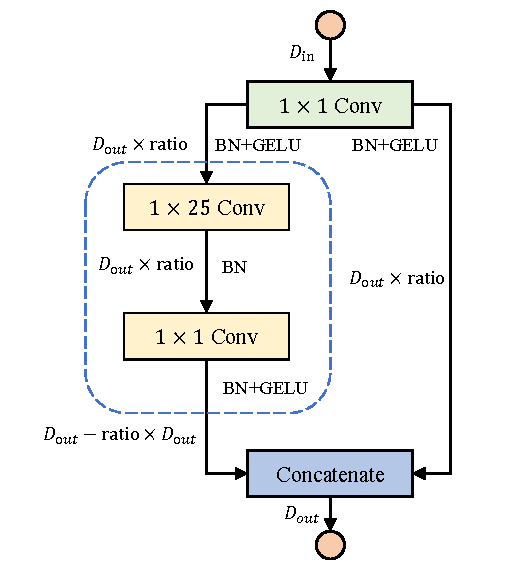
\includegraphics[width=0.5\textwidth]{SGv2.pdf}
    \caption{SG模块结构}
    \label{fig:sg}
\end{figure}

对于SG模块,论文对廉价变换卷积层做了如下改进:根据采样频率特性调整卷积核大小,为了描述的简洁性,以时间域特征提取卷积模块为例,并将其卷积核大小设定为\(1 \times 25\),对于采样频率为250Hz的BCI Competition IV Dataset 2A数据集而言,意味着该卷积核以0.1秒的时间窗口进行特征捕获。在廉价变换卷积层,特征图首先以\(1 \times 25\)可分离卷积进行特征提取,不改变特征图数量;随后经过批归一化层,使用\(1 \times 1\)逐点卷积进行特征图之间的交互,改变特征图数量;最后,经过批归一化层与GELU激活函数。

廉价变换卷积层的输入特征图数量为\(D_{out} \times ratio\),输出特征图数量为\(D_{out}-D_{out} \times ratio\),以保证输出特征图数量无偏差,由标准卷积直接传递而来的输出特征图数量为\(D_{out} \times ratio\),所有特征图在深度维度进行聚合,获得最终的输出。

\section{本章小结}